% Created 2020-09-06 Sun 13:53
% Intended LaTeX compiler: pdflatex
\documentclass[11pt]{article}
\usepackage[utf8]{inputenc}
\usepackage[T1]{fontenc}
\usepackage{graphicx}
\usepackage{grffile}
\usepackage{longtable}
\usepackage{wrapfig}
\usepackage{rotating}
\usepackage[normalem]{ulem}
\usepackage{amsmath}
\usepackage{textcomp}
\usepackage{amssymb}
\usepackage{capt-of}
\usepackage{hyperref}
\author{rodri}
\date{\today}
\title{}
\hypersetup{
 pdfauthor={rodri},
 pdftitle={},
 pdfkeywords={},
 pdfsubject={},
 pdfcreator={Emacs 28.0.50 (Org mode 9.3.7)}, 
 pdflang={English}}
\begin{document}

\tableofcontents


\documentclass[12pt,spanish,fleqn,openany,letterpaper,pagesize]{report}

% \usepackage[ansinew]{inputenc}
% \usepackage[spanish,es-tabla]{babel}
\usepackage{fancyhdr}
\usepackage{epsfig}
\usepackage{epic}
\usepackage{eepic}
\usepackage{amsmath}
\usepackage{threeparttable}
\usepackage{amscd}
\usepackage{here}
\usepackage{graphicx}
\usepackage{lscape}
\usepackage{tabularx}
\usepackage{subfigure}
\usepackage{longtable}
\usepackage{geometry}
\usepackage{pgfplots}

\usepackage{rotating} %Para rotar texto, objetos y tablas seite. No se ve en DVI solo en PS. Seite 328 Hundebuch
                        %se usa junto con \rotate, \sidewidestable ....


\renewcommand{\theequation}{\thechapter-\arabic{equation}}
\renewcommand{\thefigure}{\textbf{\thechapter-\arabic{figure}}}
\renewcommand{\thetable}{\textbf{\thechapter-\arabic{table}}}


\pagestyle{fancyplain}%\addtolength{\headwidth}{\marginparwidth}
\textheight22.5cm \topmargin0cm \textwidth16.5cm
\oddsidemargin0.5cm \evensidemargin-0.5cm%
\renewcommand{\chaptermark}[1]{\markboth{\thechapter\; #1}{}}
\renewcommand{\sectionmark}[1]{\markright{\thesection\; #1}}
\lhead[\fancyplain{}{\thepage}]{\fancyplain{}{\rightmark}}
\rhead[\fancyplain{}{\leftmark}]{\fancyplain{}{\thepage}}
\fancyfoot{}
\thispagestyle{fancy}%


\addtolength{\headwidth}{0cm}
\unitlength1mm %Define la unidad LE para Figuras
\mathindent0cm %Define la distancia de las formulas al texto,  fleqn las descentra
\marginparwidth0cm
\parindent0cm %Define la distancia de la primera linea de un parrafo a la margen

%Para tablas,  redefine el backschlash en tablas donde se define la posici\'{o}n del texto en las
%casillas (con \centering \raggedright o \raggedleft)
\newcommand{\PreserveBackslash}[1]{\let\temp=\\#1\let\\=\temp}
\let\PBS=\PreserveBackslash

%Espacio entre lineas
\renewcommand{\baselinestretch}{1.1}

%Neuer Befehl f\"{u}r die Tabelle Eigenschaften der Aktivkohlen
\newcommand{\arr}[1]{\raisebox{1.5ex}[0cm][0cm]{#1}}

%Neue Kommandos
\usepackage{Befehle}


%Trennungsliste
\hyphenation {Reaktor-ab-me-ssun-gen Gas-zu-sa-mmen-set-zung
Raum-gesch-win-dig-keit Durch-fluss Stick-stoff-gemisch
Ad-sorp-tions-tem-pe-ra-tur Klein-schmidt
Kohlen-stoff-Mole-kular-siebe Py-rolysat-aus-beu-te
Trans-port-vor-gan-ge}
\%\includeonly{Kap1/Kap1,Kap2/Kap2}
\usepackage{titlesec} 
\renewcommand{\tablename}\{\textbf{Tabla}\}
\renewcommand{\figurename}\{\textbf{Figura}\}
\renewcommand{\listtablename}{Lista de Tablas}
\renewcommand{\listfigurename}{Lista de Figuras}
\renewcommand{\labelitemi}{$\bullet$}
\titleformat{\chapter}[display]
\{\bfseries\Large\}
\{\filright\MakeUppercase{\chaptertitlename} \Huge\thechapter\}
\{1ex\}
\{\titlerule\vspace{1ex}\filleft\}
[\vspace{1ex}\titlerule]


\begin{document}

	
\pagenumbering{roman}
%\newpage
%\setcounter{page}{1}
\begin{center}
\begin{figure}
\centering%
\textsc{\large UNIVERSIDAD CAT\'OLICA BOLIVIANA ``SAN PABLO'' }\\[0.3cm] % Name of your university/college
\textsc{\large UNIDAD ACAD\'EMICA REGIONAL LA PAZ}\\[0.3cm] %
\textsc{\large FACULTAD DE INGENIER\'IA}\\[0.3cm]
\textsc{\normalsize  CARRERA DE INGENIER\'IA MECATR\'ONICA}\\[0.1cm]

\epsfig{file=HojaTitulo/UCBSinFondo.png,scale=0.75}%
\end{figure}
\textbf{\large
T\'ITULO DEL PROYECTO DE GRADO}\\[0.5cm]

\thispagestyle{empty} \vspace*{0.01cm} \textbf{\large Proyecto de grado presentado para la obtenci\'on del Grado de Ingenier\'ia Mecatr\'onica}\\[0.65cm]

\thispagestyle{empty} \vspace*{0.01cm} \normalsize Por: RODRIGO MENDOZA TEJADA SEBASTI\'AN  \\[0.8cm]

\thispagestyle{empty} \vspace*{0.01cm} \normalsize Tutor: JOHN ORDONEZ\\[1.5cm]

\vspace*{0.01cm} \normalsize La Paz-Bolivia\\[0.25cm]
\vspace*{0.01cm} \normalsize Mes, 2020
\end{center}

\newpage{\pagestyle{empty}\cleardoublepage}

\newpage

\newpage{\pagestyle{empty}\cleardoublepage}

\newpage
\thispagestyle{empty} \textbf{}\normalsize
\\\\\\%
\textbf{DEDICATORIA}\\[4.0cm]

\begin{flushright}
\begin{minipage}{8cm}
    \noindent
        \small
        La dedicatoria es opcional y cada autor podr\'a determinar la distribuci\'on del texto en la p\'{a}gina, se sugiere esta presentaci\'on. En ella el autor dedica su trabajo en forma especial a personas y/o entidades.\\[1.0cm]\\
        Por ejemplo:\\[1.0cm]
        A mis padres\\[1.0cm]\\
        o\\[1.0cm]
        La preocupaci\'on por el hombre y su destino siempre debe ser el
        inter\'es primordial de todo esfuerzo t\'ecnico. Nunca olvides esto
        entre tus diagramas y ecuaciones.\\\\
        Albert Einstein\\
\end{minipage}
\end{flushright}

%\newpage{\pagestyle{empty}\cleardoublepage}

\newpage
\thispagestyle{empty} \textbf{}\normalsize
\\\\\\%
\textbf{AGRADECIMIENTOS}
%\addcontentsline{toc}{chapter}{\numberline{}Agradecimientos}\\\\
\\\\
Esta secci\'{o}n es opcional, en ella el autor agradece a las personas o instituciones que colaboraron en la realizaci\'{o}n de la tesis  o trabajo de investigaci\'{o}n. Si se incluye esta secci\'{o}n, deben aparecer los nombres completos, los cargos y su aporte al documento.\\

\newpage{\pagestyle{empty}\cleardoublepage}

\newpage
\textbf{\LARGE Resumen}\\\\
%\addcontentsline{toc}{chapter}{\numberline{}Resumen}
\\\\
El resumen es una presentaci\'{o}n abreviada y precisa (la NTC 1486 de 2008 recomienda revisar la norma ISO 214 de 1976). Se debe usar una extensi\'{o}n m\'{a}xima de 15 renglones. Se recomienda que este resumen sea anal\'{\i}tico, es decir, que sea completo, con informaci\'{o}n cuantitativa y cualitativa, generalmente incluyendo los siguientes aspectos: objetivos, dise\~{n}o, lugar y circunstancias, objetivo del estudio, intervenci\'{o}n, mediciones y principales resultados, y conclusiones. Al final del resumen se deben usar palabras claves tomadas del texto (m\'{\i}nimo 3 y m\'{a}ximo 7 palabras), las cuales permiten la recuperaci\'{o}n de la informaci\'{o}n.\\

\textbf{\small \textit{Palabras clave: (m\'{a}ximo 10 palabras, preferiblemente seleccionadas de las listas internacionales que permitan el indizado cruzado)}}.\\

\textbf{\small L\'inea de investigaci\'on:} \small (m\'aximo 1 o 2  rengl\'ones en que se establezca la  l\'inea de investigaci\'on a la que pertenece el proyecto de grado).\\


\newpage
\textbf{\LARGE Abstract}\\\\
Es el mismo resumen pero traducido al ingl\'{e}s. Se debe usar una extensi\'{o}n m\'{a}xima de 12 renglones. Al final del Abstract se deben traducir las anteriores palabras claves tomadas del texto (m\'{\i}nimo 3 y m\'{a}ximo 7 palabras), llamadas keywords. Es posible incluir el resumen en otro idioma diferente al espa\~{n}ol o al ingl\'{e}s, si se considera como importante dentro del tema tratado en la investigaci\'{o}n, por ejemplo: un trabajo dedicado a problemas ling\"{u}\'{\i}sticos del mandar\'{\i}n seguramente estar\'{\i}a mejor con un resumen en mandar\'{\i}n.\\[2.0cm]
\textbf{\small \textit {Keywords: palabras clave en ingl\'es(m\'aximo 10 palabras, preferiblemente seleccionadas de las listas internacionales que permitan el indizado cruzado)}}\\

\textbf{\small Research area:} \small texto en ingl\'es (m\'aximo 1 o 2
rengl\'ones en que se establezca la  l\'inea de investigaci\'on a la que
pertenece el proyecto de grado).\\
%%% Local Variables:
%%% mode: latex
%%% TeX-master: "../TesisMSc"
%%% End:


\renewcommand{\contentsname}{\textbf{\LARGE \'Indice}}


%\chapter*{Lista de s\'imbolos}
%\textbf{\Large Lista de s\'imbolos} \\\\
\textbf{\LARGE Notaci\'on}\\\\
%\lhead{\emph{Lista de s\'imbolos}}
%\addcontentsline{toc}{chapter}{\numberline{}Lista de s\'{\i}mbolos}
Esta secci\'{o}n es opcional, dado que existen disciplinas que no manejan s\'{\i}mbolos y/o abreviaturas.\\

Se incluyen s\'{\i}mbolos generales (con letras latinas y griegas), sub\'{\i}ndices, super\'{\i}ndices y abreviaturas (incluir s\'{o}lo las clases de s\'{\i}mbolos que se utilicen). Cada una de estas listas debe estar ubicada en orden alfab\'{e}tico de acuerdo con la primera letra del s\'{\i}mbolo.
%\section*{S\'{\i}mbolos con letras latinas}
 \label{simbolos}
 \renewcommand{\arraystretch}{1.3}
%\begin{longtable}[l]{*{4}{>{$}l<{$}}p{9cm}}
%\begin{longtable}[l]{>{$}l<{$}l>{$}l<{$}>{$}l<{$}}
\begin{longtable}[l]{>{$}l<{$}l>{$}l<{$}}
%\begin{tabular}
\textbf{S\'{\i}mbolo}&\textbf{T\'{e}rmino}&\\[0.6ex]\hline
\endfirsthead%
\textbf{S\'{\i}mbolo}&\textbf{T\'{e}rmino}&\\[0.6ex]\hline
\endhead%
      I_{\text{max}}        & Corriente m\'axima[\textit A]                                                  \\%
      \alpha &tasa de aprendizaje                     \\%
      \lambda_{\text{i}}   & Autovalor i                             \\%

\end{longtable}
\vspace{5ex}



\section*{Glosario}
\begin{longtable}[l]{>{}l<{}l}
  \textbf{Abreviatura} & \textbf{T\'{e}rmino} \\[0.5ex] \hline%
  \endfirsthead%
  \textbf{Abreviatura} & \textbf{T\'{e}rmino} \\[0.5ex] \hline%
  \endhead%
\renewcommand{\arraystretch}{1.4}\label{simbolosg}
 $DP$&Deep Learning - Aprendizaje profundo \\%
 $FCEM$    & Fuerza contraelectromotriz\\%
 $RAM$   &Random Access Memory - Memoria de Acceso Aleatorio\\%

\end{longtable}


\setlength{\extrarowheight}{0pt}
%\newcommand{\clearemptydoublepage}{\newpage{\pagestyle{empty}\cleardoublepage}}


\tableofcontents
\listoffigures

\listoftables
%\include{Resumen}%\newcommand{\clearemptydoublepage}{\newpage{\pagestyle{empty}\cleardoublepage}}
\newpage
\pagenumbering{arabic}
% \chapter{Marco Referencial}

\section{Introducción}
\label{sec:orga059c5a}
Las bioseñales son originadas por la actividad eléctrica generada por un ser viviente. Estas pueden ser impulsos eléctricos enviados a los músculos para contracción, así como los generados por las sinapsis del cerebro. Las señales más conocidas y estudiadas son: las provenientes del corazón (ECG\footnote{ECG, por sus siglas en inglés: Electrocardiography}), del movimiento intraocular (EOG\footnote{EOG, por sus siglas en inglés: Electrooculography}), del movimiento muscular (EMG\footnote{EMG, por sus siglas en inglés: Electromyogram}) y de la actividad cerebral (EEG\footnote{EEG, por sus siglas en inglés: Electroencephalography}).

Estas señales\footnote{BCI, por sus siglas en inglés: Brain-Computer Interface\label{org2010a5c}} pueden ser medidas por medio de electrodos colocados en la superficie de piel más cercana al origen del impulso eléctrico. Sin embargo, este método presenta grandes problemas con el ruido considerando que este, puede provenir de la carga electroestática que se encuentre sobre la piel o pelo en el área de contacto. Adicionalmente, se presentan muchos artefactos, señales que no están relacionadas a la señal de interés \cite{I.R.KeckV.FischerC.G.Puntonet2011} [6]; tanto de origen biológico como no biológico.
asdf

En las bioseñales, los artefactos presentes suelen ser de la misma o incluso mayor magnitud que la señal de interés. Una forma de evitar estas interferencias es emplear amplificadores diferenciales como parte del diseño electrónico del dispositivo de adquisición [17]. Pero además, en conjunto, se utiliza una cantidad de electrodos elevada para reducir los artefactos y colocarlos en disposiciones específicas según el caso de uso [8].
Por otro lado, existen dos tipos de usuarios que emplean y manipulan dispositivos de adquisición de bioseñales o BAS\footnote{BAS, por sus siglas en inglés: Biosignal Acquisition System}:

\begin{itemize}
\item Investigadores y desarrolladores de tecnologías. Estos emplean los dispositivos BAS para crear interfaces con computadores que asocian patrones en las bioseñales con intenciones del usuario. Cada asociación puede servir como un canal de entrada para la interfaz. Generalmente se realiza el uso de EEG para crear una BCI\textsuperscript{\ref{org2010a5c}} Interfaz Cerebro-Computador. En esta aplicación, pueden haber asociaciones de actividades cerebrales con intenciones creando múltiples canales de entrada para la interfaz desarrollada. Por ejemplo, un sistema BCI puede reconocer actividad cerebral motora (MI - Motor Imagery) de la mano izquierda y derecha [4]; de este modo, se pueden asociar estas dos actividades como dos entradas para una interfaz.

\item Practicantes de ciencias como la medicina y psicología para el diagnóstico, rehabilitación, monitoreo; así como estudio de la naturaleza y comportamiento de las señales. En el caso de la medicina, puede ser crítico en algunos casos. Un ejemplo es el monitoreo de la presencia de actividad cerebral en pacientes en coma [14]. En otros casos puede ser utilizados en estudios de polisomnografía para diagnosticar enfermedades o trastornos en el sueño.
\end{itemize}

Cabe mencionar que todos los casos de uso se ven afectados por la cantidad de canales disponibles para la medición de ondas cerebrales. Esto se debe a que en un evento, la actividad cerebral se propaga en múltiples direcciones desde su origen. Por lo que, a medida que mayor sea la cantidad de electrodos utilizados se podrá captar mejor el evento. Una evidencia de esto se presenta en los estudios de polisomnografía \cite{Bubrick2014} [2].

\section{Planteamiento del Problema}
\label{sec:org3aff47d}
De todas las bioseñales, la EEG presenta las mayores dificultades ya que la magnitud de la señal que puede llegar a estar varios órdenes por debajo del ruido y también de los artefactos; esto indica que la relación SNR\footnote{SNR, por sus siglas en inglés: Signal to Noise Ratio} señal-ruido en condiciones normales es la más baja entre las bioseñales. Por este motivo acompañado de la gran similitud entre las bioseñales, un dispositivo que sea capaz de medir una señal EEG es capaz de medir las otras mencionadas anteriormente [1]. Podemos observar cómo esto es posible si nos enfocamos en tres características de cualquier señal: frecuencia, magnitud y SNR.

Debido a la naturaleza analógica y el diseño in-expansible, los dispositivos cuentan con muchas limitaciones en cuanto a potenciación si no se elimina al financiamiento como un factor determinante. Como efecto, dificulta la generación de variantes más económicas que se ajusten a distintos tipos de aplicación.

Finalmente, en el lado del software, los dispositivos comerciales suelen brindar actualizaciones de firmware que puedan optimizar el funcionamiento a través de filtros digitales así como otros algoritmos de manejo de datos. Este procedimiento de actualización es trivial y no presentan mayores complicaciones debido a que las versiones suelen ser estables, permitiendo obviar las actualizaciones sin causar mayores complicaciones. Sin embargo, los distintos dispositivos cuentan con distintos software propietarios causando una gran incompatibilidad entre los dispositivos. Existen software como EEGLAB y BCILAB [22] que son compatibles con algunos de los dispositivos de medición de bioseñales EEG, sin embargo están programados sobre intermediarios como MATLAB. Otros como el OpenBCI [21] y OpenVibe [25] permiten compatibilidad con lenguajes y tecnologías más modernas; pero la compatibilidad se mantiene muy limitada ya que requiere que el usuario programe.

\subsection{Definición del problema}
\label{sec:org88e0b95}
Actualmente hay baja disponibilidad en el mercado de dispositivos para la medición de multiples bioseñales que además sean asequibles para investigadores independientes. Asimismo es baja la variedad en los proyectos Open Source relacionados. Esto supone una brecha en el conocimiento e investigación de la neurociencia ya que hay un costo elevado para la inmersión en ésta práctica.

\section{Objetivos}
\label{sec:org3643799}
\subsection{Objetivo General}
\label{sec:orgce1e4b4}
Implementar un sistema modular que permita medir y grabar digitalmente bioseñales EEG.

\subsection{Objetivos específicos}
\label{sec:orgec72373}
\begin{itemize}
\item Desarrollar un sistema para la medición digital 2 canales simultáneos e independientes de señales EEG.
\item Implementar 1 canal independiente de referencia.
\item Validar la calibración con una señal de onda cuadrada a 100uVpp, 10Hz.
\item Validar las mediciones de EEG según su forma y frecuencia en base a la comparativa con mediciones realizadas por otros dispositivos.
\item Implementar el sistema con forma modular.
\item Diseñar un sistema de protección contra descargas electroestáticas.
\item Desarrollar una interfaz intuitiva, cuyo uso no requiera conocimientos de programación.
\item Implementar un sistema de comunicación de datos a través de WiFi.
\end{itemize}

\section{Justificación}
\label{sec:org10a5754}
El proyecto se ve entonces justificado con motivo de reducir la brecha de conocimiento al proveer de una alternativa mas flexible en el aspecto económico limitando más adecuadamente el sacrificio en el desempeño. En un punto de vista conceptual brindará un formato mas sencillo y práctico para entender los conceptos de la electroencefalografía y neurociencia. En el área técnica, se genera un diseño simple de reproducir beneficiando a las aplicaciones vecinas que puedan aprovechar sus fortalezas. Del punto de vista académico el aporte es interdisciplinario, uniendo conceptos de sistemas informáticos como el ser redes de comunicación y bases de datos con sistemas de computación embebidos. Asimismo, se le suma el diseño de un dispositivo de adquisición de señales analógicas a digitales con una precisión y robustez muy elevada.

\section{Límites y Alcances}
\label{sec:orgf901299}
\subsection{Límites}
\label{sec:org12a460e}
\begin{itemize}
\item Publicar el código con las instrucciones reservadas únicamente para la implementación en MacOS Catalina.
\item Cumplimiento de requerimientos estrictamente referentes la calibración en el subtitulo 3 y la grabación en los subtítulos 4 y 5 puestos por la IFCN para la medición clínica digital de EEG [7].
\item Comprobar si el sistema puede soportar hasta 24 canales desde un enfoque teórico.
\item Implementar únicamente los módulos necesarios para cumplir los requerimientos mencionados para la medición clínica digital de señales EEG.
\item Manufacturar una copia única de cada módulo.
\item Código desarrollado solo para el micro-controlador ESP32 en Arduino.
\end{itemize}

\subsection{Alcances}
\label{sec:org8df9321}
\begin{itemize}
\item Proporcionar los diseños y breves manuales en repositorios cómo GitHub con una licencia de código abierto sobre el contenido.
\item Diseño modular con compatibilidad con EEG, ECG, EMG, EOG al variar la magnitud de amplificación, reemplazo de filtros.
\item El sistema original implementado medirá hasta 2 canales digitales; sin embargo el sistema debe ser capaz de aumentar el número de entradas con el intercambio o adición de nuevos módulos.
\item Tanto la configuración inicial como el uso del dispositivo se deben poder llevar a cabo sin conocimientos en lenguajes de programación o muy avanzados en computación.
\item El sistema debe contar con protección de descargas electroestáticas (ESD) sobre el circuito.
\item El sistema debe contar con protección desde la fuente de alimentación; esta debe ser al menos de 1kV por 1s a través de un aislamiento galvánico y como alternativa el funcionamiento independiente a base de baterías.
\end{itemize}

\section{export\textsubscript{latex}}
\label{sec:org1fa961e}
\begin{verbatim}
%%% Local Variables:
%%% mode: latex
%%% TeX-master: "../TesisMSc"
%%% End:
\end{verbatim}


\chapter{Marco Referencial}
\section{Introducción}
Mi nómbre es pepitó

hellooooooo.\\

En la introducci\'{o}n, el autor presenta y se\~{n}ala la importancia, el origen (los antecedentes te\'{o}ricos y pr\'{a}cticos), los objetivos, los alcances, las limitaciones, la metodolog\'{\i}a empleada, el significado que el estudio tiene en el avance del campo respectivo y su aplicaci\'{o}n en el \'{a}rea investigada. No debe confundirse con el resumen y se recomienda que la introducci\'{o}n tenga una extensi\'{o}n de m\'{\i}nimo 2 p\'{a}ginas y m\'{a}ximo de 4 p\'{a}ginas.\\

La presente plantilla maneja una familia de fuentes utilizada generalmente en LaTeX, conocida como Computer Modern, espec\'{\i}ficamente LMRomanM para el texto de los p\'{a}rrafos y CMU Sans Serif para los t\'{\i}tulos y subt\'{\i}tulos. Sin embargo, es posible sugerir otras fuentes tales como Garomond, Calibri, Cambria, Arial o Times New Roman, que por claridad y forma, son adecuadas para la edici\'{o}n de textos acad\'{e}micos.\\

La presente plantilla tiene en cuenta aspectos importantes de la Norma T\'{e}cnica Colombiana - NTC 1486, con el fin que sea usada para la presentaci\'{o}n final de las tesis de maestr\'{\i}a y doctorado y especializaciones y especialidades en el \'{a}rea de la salud, desarrolladas en la Universidad Nacional de Colombia.\\

Las m\'{a}rgenes, numeraci\'{o}n, tama\~{n}o de las fuentes y dem\'{a}s aspectos de formato, deben ser conservada de acuerdo con esta plantilla, la cual esta dise\~{n}ada para imprimir por lado y lado en hojas tama\~{n}o carta. Se sugiere que los encabezados cambien seg\'{u}n la secci\'{o}n del documento (para lo cual esta plantilla esta construida por secciones).\\

Si se requiere ampliar la informaci\'{o}n sobre normas adicionales para la escritura se puede consultar la norma NTC 1486 en la Base de datos del ICONTEC (Normas T\'{e}cnicas Colombianas) disponible en el portal del SINAB de la Universidad Nacional de Colombia\footnote{ver: www.sinab.unal.edu.co}, en la secci\'{o}n "Recursos bibliogr\'{a}ficos" opci\'{o}n "Bases de datos".  Este portal tambi\'{e}n brinda la posibilidad de acceder a un instructivo para la utilizaci\'{o}n de Microsoft Word y Acrobat Professional, el cual est\'{a} disponible en la secci\'{o}n "Servicios", opci\'{o}n "Tr\'{a}mites" y enlace "Entrega de tesis".\\

La redacci\'{o}n debe ser impersonal y gen\'{e}rica. La numeraci\'{o}n de las hojas sugiere que las p\'{a}ginas preliminares se realicen en n\'{u}meros romanos en may\'{u}scula y las dem\'{a}s en n\'{u}meros ar\'{a}bigos, en forma consecutiva a partir de la introducci\'{o}n que comenzar\'{a} con el n\'{u}mero 1. La cubierta y la portada no se numeran pero si se cuentan como p\'{a}ginas.\\

Para trabajos muy extensos se recomienda publicar m\'{a}s de un volumen. Se debe tener en cuenta que algunas facultades tienen reglamentada la extensi\'{o}n m\'{a}xima de las tesis  o trabajo de investigaci\'{o}n; en caso que no sea as\'{\i}, se sugiere que el documento no supere 120 p\'{a}ginas.\\

No se debe utilizar numeraci\'{o}n compuesta como 13A, 14B \'{o} 17 bis, entre otros, que indican superposici\'{o}n de texto en el documento. Para resaltar, puede usarse letra cursiva o negrilla. Los t\'{e}rminos de otras lenguas que aparezcan dentro del texto se escriben en cursiva.\\

\section{Planteamiento del Problema}
\subsection{Definici\'on del problema}

\section{Objetivos}
\subsection{Objetivo General}
\subsection{Objetivos espec\'ificos}
\begin{itemize}
	
	\item Objetivo espec\'ifico 1 
	\item Objetivo espec\'ifico 2 
	\item Objetivo espec\'ifico 3 
	\item Objetivo espec\'ifico 4 
	\item Objetivo espec\'ifico 5 
	\item Objetivo espec\'ifico 6 
\end{itemize}


\section{Justificaci\'on}
\section{L\'imites y Alcances}
\subsection{L\'imites}
\begin{itemize}
	
	\item L\'imite 1 
	\item L\'imite 2 
	\item L\'imite 3 
	\item L\'imite 4 
	\item L\'imite 5 
	\item L\'imiteo 6 
\end{itemize}
\subsection{Alcances}

\begin{itemize}
	
	\item Alcance 1 
	\item Alcance 2
	\item Alcance 3
	\item Alcance 4
	\item Alcance 5
	\item Alcance 6
\end{itemize}

%%% Local Variables:
%%% mode: latex
%%% TeX-master: "../TesisMSc"
%%% End:

\chapter{Marco Teórico}\\

\section{Estado del Arte}
\label{sec:orgc709def}
\texttt{La electroencefalografía (EEG) es un estudio que se basa en la interpretación de los impulsos eléctricos producidos por las neuronas.}\\

\texttt{, que se utiliza para detectar anomalías en los patrones de ondas producidas por el cerebro.}\\

\texttt{Esta práctica tiene una larga trayectoria con un alza reciente en el interés por crear interfaces que permitan conectar actividades cerebrales con entradas a un computador denominadas BCI por sus siglas en inglés ‘Brain-Computer Interface’. Hoy en dia hablamos de un gran alza en BCI proyectando alcanzar \$1.46 billones de dolares en el mercado para el 2020 [1].}\\

Motivados por esto, los fabricantes de circuitos integrados han logrado captar las necesidades del mercado proveyendo alternativas que logran simplificar el proceso, mejorando el rendimiento y reduciendo el costo global. Así mismo, podemos decir que se ha roto la barrera de acceso a estos dispositivos en el mercado comercial gracias a la evolución de la tecnología, permitiendo desarrollar dispositivos de mucha complejidad con costos muy bajos, nunca antes visto en esta industria.\\

Esto a generado necesidad de contar con dispositivos para mediciones EEG más competitivos en todas las áreas que, en ultima instancia, resulta en gran beneficio para el crecimiento de la neurociencia en general. Hoy en día, hay implementaciones interesantes de dispositivos portatiles [1], en formas poco convencionales y con varios tipos de sensores. Por ello ha sido evidente el beneficio de toda la comunidad relacionada al área; pues, se ha visto expuesta a poderosos dispositivos que pasan de circuitos extensos y un procesamiento analógico complejo, a un arreglo simple de circuitos integrados apoyados por un fuerte procesamiento digital. Aun así, el mercado presenta pocas opciones disponibles para los que pretenden integrarse en esta ciencia.\\

Para el desarrollo de tales dispositivos se deben contemplar varias consideraciones: Seguridad para el paciente, resolución de la señal, movilidad del dispositivo para ser trasladado fácilmente, costo y escalabilidad entre otros. Debemos observar el estado del arte actual enfocándonos en temas más técnicos. El siguiente diagrama de bloques presentado en la figura 1 nos muestra los componentes de un dispositivo EEG genérico.\\

\begin{figure}[htbp]
\centering
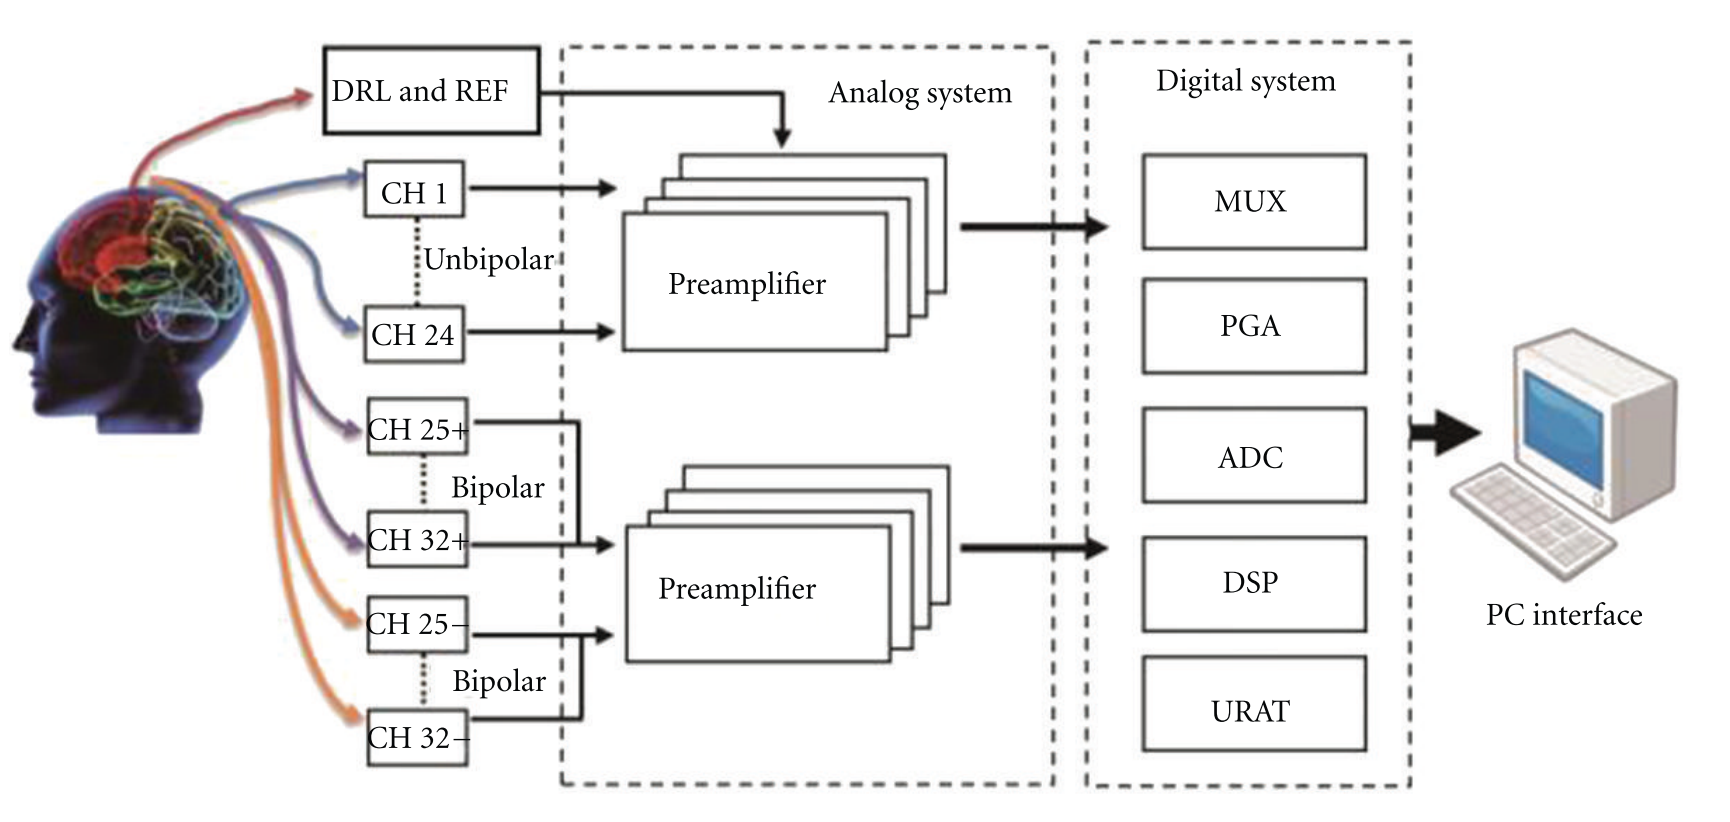
\includegraphics[width=.9\linewidth]{Kap2/bloques_EEG.png}
\caption{\label{fig:bloques_eeg}Diagrama de bloques de un dispositivo EEG Genérico}
\end{figure}

Observamos un primer bloque compuesto por los electrodos. La investigación existente sobre el funcionamiento y la tipología de los electrodos es muy extensa y profunda. De hecho, ahondar en ello llevaría la totalidad del documento.\\

El segundo bloque es el procesamiento analógico. Si bien se ha observado el decremento de la importancia y tamaño de esta parte, aún es imprescindible en los diseños antes de poder entrar al mundo digital.\\

Lógicamente el tercer bloque es el diseño digital. Esto involucra todo lo que conlleva el muestreo, pre-procesamiento, transmisión, almacenamiento y post procesamiento de la señal. En si, esta área es poco definida ya que puede ser fácilmente reconfigurada por medio de una actualización de código.\\

El cuarto bloque engloba a todo el sistema y es sin duda uno de los más importantes; Es la protección eléctrica. Como veremos mas adelante, existen muchos riesgos y consideraciones que deben ser los pilares para todo diseño de dispositivos para la medición de bio-señales.\\

A continuación se describe cada una de estas áreas o componentes, en un orden medio jerárquico:\\

\subsection{Protección eléctrica}
\label{sec:org9805377}
Como se comentó previamente, este bloque concierne a todos los demás, por lo cual se describe en primer lugar, a pesar de que en el proceso no es la “primer etapa”, si es que se pudiera dar un orden de secuencia al proceso.\\

La importancia de este punto yace en que este tipo de dispositivos, operan directamente con seres humanos. Por lo que en primer lugar se debe garantizar la seguridad antes de cualquier consideración técnica o de costo. Por otro lado, también debe poder garantizarse la estabilidad y fiabilidad del circuito, pues de lo contrario ningún resultado sería confiable.\\

\subsubsection{ESD}
\label{sec:org73b57f2}
Los circuitos integrados son el corazón de casi todos los circuitos electrónicos actuales. El inconveniente con estos dispositivos se debe a que algunos son altamente sensibles a descargas electrostáticas (ESD) por contacto directo o por transmisión desde otra localización de el circuito.\\

Para el primer caso (contacto directo) existen dos métodos básicos que se implementan a lo largo de la industria.\\

\begin{itemize}
\item Utilizar un contenedor de un material no conductor que genere un aislamiento galvánico entre el circuito y el usuario; Esto es una separación física entre ambos. Evidentemente, esto aumenta la resiliencia, movilidad y estética del dispositivo en general. Como punto aparte se pudiera recomendar la implementación de una capa conductora en el exterior del contenedor que sirva como aislante EMI\footnote{EMI, por sus siglas en inglés: \emph{Electro Magnetic Interferences}\\} del ambiente. En el subtitulo 2.2.1 se explicarán los motivos de esta última recomendación con mucho más detalle.\\

\item Incluir señalizaciones adecuadas sobre estos riesgos y cual debe ser la correcta manipulación del equipo. Las señalizaciones deben ir pertinentemente en el circuito, el contenedor y los manuales del dispositivo. Es imprescindible alertar al usuario de los riesgos presentes que corre tanto el circuito como él mismo.\\
\end{itemize}

Ahora bien, el segundo caso (transmisión indirecta) o fuente de riesgo, proviene de los electrodos. Debemos tomar en cuenta tres factores:\\
\begin{itemize}
\item Las personas suelen acumular carga estática sobre la piel\\
\item La función principal de los electrodos es transmitir corriente eléctrica\\
\item En aplicaciones de EEG se recomienda utilizar una alta densidad de electrodos (24 electrodos o más).\\
\end{itemize}

El dispositivo queda continuamente sometido a varias descargas eléctricas de baja potencia y potencialmente sometido a descargas cortas de alto voltaje. Este peligro al circuito es inevitable, pues es muy difícil remover toda carga estática sobre una persona. Sin embargo, existen varios métodos para reducir el peligro, que van desde reducir el nivel de acumulación de carga del usuario, hasta incrementar la resiliencia del circuito ante una descarga eléctrica.\\

Para el primer caso (contacto directo) existen métodos como el DRL\footnote{DRL, por sus siglas en inglés: \emph{Driven Right Leg}\\} \cite{Winter1983} que busca nivelar las cargas presentes sobre el usuario al inducir una carga opuesta. Éste método será explicado en el subtítulo 2.1.2 ya que su principal beneficio se muestra mayormente en la reducción de ruido y no tanto así en ésta área.\\

El segundo caso (transmisión indirecta) es imprescindible ya que la eficiencia de los otros métodos puede variar. Los método comúnmente usado es la implementación de un arreglo de diodos que lleven descargas peligrosas al plano de tierra. Este método mejora así la resiliencia general del circuito.\\

En resumen, es esencial contar con una capa de protección entre los electrodos y el dispositivo. Esto se logra de dos formas: Primero, generando una impedancia de entrada muy alta que sirva de barrera inicial. Segundo, implementando un arreglo de diodos en la entrada que proteja el circuito de cualquier exceso de carga. Generalmente los cables de los electrodos no se encuentran soldados al circuito por lo cual es común ver esta capa de protección justo al lado de los conectores.\\

\subsubsection{Transmisión de datos}
\label{sec:org6bb3188}
El dispositivo debe ser capaz de medir, grabar y mostrar las mediciones de las señales en vivo. Por consiguiente, es necesario incluir un visualizador en la interfaz con el usuario. Esta interfaz puede estar integrada en el dispositivo, puede ser una computadora anexada al mismo de manera permanente o temporal. De igual forma el dispositivo puede ser dependiente o independiente de dicha computadora. Para determinar la alternativa más adecuada podemos considerar los siguientes factores según el tipo de aplicación:\\

\begin{enumerate}
\item Móvil o estacionaria. Esto nos va a permitir determinar inmediatamente una transmisión de datos inalámbrica y fuente de alimentación por baterías.\\
\item Longitud de sesión de medición. En aplicaciones que se requiera un monitoreo extenso como lo es el de la polisomnografía observamos claramente que es esencial una autonomía de 8-10 horas. Esto nos limita las opciones de baterías dejando como favorito a una alimentación de linea directa.\\
\end{enumerate}

A modo de no sobrecargar la alimentación aislada que conseguimos con los conversores DC- DC o las baterías, podemos crear otro sistema con una alimentación independiente.\\

Sin embargo, en todas las aplicaciones observamos que la transmisión de datos para la visualización en vivo debe ser aislada galvánicamente. Por tanto podemos utilizar un método de aislamiento basado en transformación de señal eléctrica en otra. Un método eficiente y directo es el uso de optocopladores que por medio de una conversión de la señal digital a luz logran el aislamiento. Otro método más común es el de la implementación de señales de radiofrecuencia como Bluetooth o WiFi.\\

\texttt{Sin embargo, se debe considerar las limitaciones en ancho de banda ya que el volumen de datos que se transmite es considerable, los cálculos exactos se vera mas adelante en \textasciitilde{}asdfadsf\textasciitilde{}. Los optocopladores a pesar de ser una integración directa y simple es muy limitada en este aspecto; así mismo es el caso del bluetooth. Éste último es preferído en el área por su bajo consumo y fácil implementación, no obstante limita el número de canales disponibles.}\\

Una mejor alternativa es la implementación de Wifi ya que su ancho de banda es mucho mas alto y tiene una estabilidad similar. Sin embargo, su implementación es compleja ya que requiere de una connexión a una red WiFi preexistente, o la generación de una propia; el consumo de energía es mayor; la implementación de software, si bien es muy flexible, es considerablemente más compleja.\\

\subsubsection{Línea de Corriente}
\label{sec:orge0e6cea}
Este es sin duda el punto mas crítico de todo el proyecto. Debido a que en esta aplicación se colocan electrodos conductores directamente en la superficie del cuero cabelludo de una persona. Aunque el riesgo es muy bajo, el peligro es máximo en caso de una descarga eléctrica proveniente de un mal funcionamiento en una linea de corriente eléctrica. Por ello se debe mitigar al máximo el peligro por medio de un aislamiento galvánico, desconexión física, entre la fuente de alimentación y el dispositivo.\\

El uso de fusibles no es viable debido a su principio de funcionamiento. Estos requieren primeramente que una potencia mas alta de su tolerancia atraviese su paso y los destruya. Por lo tanto, la descarga de alta potencia pudiera atravesar el fusible antes de que este se quiebre, así haciéndose paso hasta el usuario.\\

Los dispositivos mas económicos optan por restringir físicamente la potencia máxima que puede presentar la fuente de energía del dispositivo con el uso de baterías. Esto tiene, además, una mayor utilidad en aplicaciones móviles. No obstante, la mayor parte de las aplicaciones médicas consisten en sesiones estacionarias y largas en muchos casos. Por lo cual esta solución no es capaz de satisfacer por si sola a todas las aplicaciones.\\

Para los casos remanentes existen dispositivos como los conversores DC-DC aislados. Similares a los conversores de corriente alterna, estos dispositivos transfieren potencial eléctrico desde una linea de corriente a través de la transformación una corriente magnética seguida de una segunda transformación a corriente eléctrica. Como resultado se genera una separación física, al menos en corriente eléctrica, poniendo una barrera lo suficientemente alta como para ser el factor de menor peligro ante una descarga eléctrica grande. Por ello, estos dispositivos se pueden encontrar en casi cualquier equipo médico con línea de alimentación fija.\\

\subsection{Procesamiento Analógico}
\label{sec:org0a9564b}
Esta es la sección que más se ha visto impactada por la sofisticación de la tecnología de ADCs y procesadores. Esto es bueno ya que permite reducir costos a la par que disminuye la complejidad de los diseños, otorgando ventajas para llegar a donde antes no se había llegado en calidad, precisión y disponibilidad para el medio. Sin embargo, como se verá en los próximos incisos a mas detalle, aún se ve el impacto positivo del procesamiento analógico.\\

La relación que existe entre la señal con el ruido del ambiente, se denomina taza de señal a ruido o SNR. Como veremos en el subtitulo C.3 del capítulo 2.2.1 (Naturaleza de la Señal) este parámetro es de gran utilidad a la hora de evaluar la calidad de la medición. Por ahora podemos mencionar que la principal misión del circuito analógico es acondicionar la señal para la digitalización a través de la mejora del SNR.\\

En esta etapa estamos considerando 3 factores principales: Ruido de Nodo Común, Offset DC y Aliasing.\\

[[imagen 1]\\

La señal primordial de \emph{ruido de nodo común} proviene de las lineas de corriente, asi tambien como otros dispositivos como luces fluorescentes pantallas y otras fuentes de ruido EMI presentes en la habitación en la que se esta realizando la medición. El \emph{Offset DC} ocurre debido a la estática acumulada sobre la piel; esta puede variar entre electrodo y electrodo. La \emph{magnitud de las señales} ECG son hasta de 5mV. Sin embargo las señales EEG miden entre 1-160µV. En este caso observamos que debemos tratar con 3 problemas; Rechazo del Ruido de Nodo Común o CMNR\footnote{CMNR: Por sus siglas en inglés: \emph{Common-Mode Noise Rejection}\\}, disminuir el desfase producido por señales DC, amplificar la señal para alcanzar una resolución de 0.5μV \cite{IFCN1999a}.\\

Finalmente debemos tomar en cuenta el concepto de solapamiento o aliasing que indica que una señal de alta frecuencia puede mostrase como señal de baja frecuencia. Este concepto nace en las inconsistencias que brotan al tratar de interpretar discretamente un sistema de tiempo continuo. Ciertamente es muy improbable que este  sea el único componente del procesamiento analógico que pueda ser remplazado completamente por un procesamiento digital, al menos no con las tecnologías comerciales actualmente disponibles.\\

\subsubsection{Driven Right Leg}
\label{sec:orgc424e14}
El circuito introducido por Bruce B.Winter y John G. Webserter en 1983 \cite{Winter1983}, es un pilar en los dispositivos profesionales de medición de cualquier bio-señal por su eficacia en la reducción de ruido. Este aporte ha demostrado su beneficio en la medición de todas las bio-señales desde su introducción en el medio. Su principio de funcionamiento propone reducir el ruido que existe sobre el usuario al inducirle una señal opuesta al electrodo de referencia. De esta manera, se logran efectos similares al aterramiento eléctrico sin poner en riesgo la eficacia de las medias de protección implementadas en el dispositivo. Una práctica común es utilizar cables coaxiales y utilizar esta señal invertida para la linea más externa. Esto reduce el ruido EMI recogido por los cables.\\

Sin embargo, su uso es escaso en dispositivos comerciales modernos. Aun así, su uso aún es fuertemente recomendado en la industria por su gran relación de costo/beneficio[4]. Esta reducción se ha dado tanto por las mejoras de los ADC como el aumento de potencia disponible para el procesamiento digital [5].\\

\subsubsection{Filtros}
\label{sec:org7dc5fd8}
Como se observa en la Figura 2, la estática existente sobre el cuerpo significa un desfase de la señal. Este desfase puede causar saturación en el sistema de muestreo. Por ello se utilizan filtros pasa altos para acondicionar la señal antes de aplicar amplificaciones grandes. En circuitos que no se utilice el DRL, el filtro pasa altos se vuelve aún mas importante ya que funge de estabilizador de la señal colocándola a nivel de tierra para evitar saturación en la etapa de amplificación. Debemos recordar que esta señal idealmente debe ser amplificada mas de 100 veces para poder obtener una buena resolución de la señal. La frecuencia de corte de este filtro, aun en la etapa digital, no debería sobrepasar 1Hz.\\

El aliasing tradicionalmente es lidiado con un filtro el cual La IFCN indica que debe estar en 70Hz con una atenuación de 12dB/dec cuando la frecuencia de muestreo es de 200 muestras por segundo (200 Hz); es decir, una proporción aproximada de 1 a 3. Esta es la configuración mínima recomendada. Las ondas electroencefalográficas pueden llegar a alcanzar 100Hz. Por lo cual si el diseño lo permite, se puede optar por un filtro en 100Hz con un muestreo de 350Hz o mayor.\\

La mejor forma de implementar filtros analógicos actualmente es por medio de filtros activos a modo de evitar la degradación de la señal. Entre estos existen dos arquitecturas principales; Sallen-Key y Multiple Feedback o MFB. En paralelo estas arquitecturas, existen 3 categorias principales de filtros distintos; Butterworth, Chebyshev, Bessel. Estas clasificaciones aplican para todos los tipos de filtros; pasa bajos, pasa altos, pasa banda, rechaza banda. En el subtítulo D del capítulo 2.2.2 (Procesamiento analógico) se ahondará en algunos de los filtros anteriormente mencionados.\\

Sin embargo todavía podemos mencionar lo siguiente respecto al tema; Mientras la arquitectura Sallen-Key presenta un número reducidos de componentes, no se recomienda para filtros pasa bajos debido a su respuesta en frecuencias altas en las que su atenuación deja de ser efectiva. La arquitectura MFB entonces es mas adecuada en esta situación. Para el filtro pasa altos entones, es recomendable una arquitectura Sallen-Key debido a su reducido número de componentes.\\

No obstante para ambos filtros se debe considerar las tolerancias de los componentes. Si bien los métodos de manufactura han logrado hitos muy importantes en la fabricación y calidad de los componentes pasivos, su sensibilidad ante cambios de temperatura y voltajes agregan complejidad a la implementación de filtros analógicos. Ahora bien, si los componentes son seleccionados aprovechando al máximo las proporciones, se puede minimizar el efecto negativo de las tolerancias.\\

\subsubsection{Amplificadores de Instrumentación}
\label{sec:orgaa33a78}
El contexto de medición de EEG nos presenta un estado donde la señal es hasta mil veces mas pequeña que el ruido proveniente del ambiente; existe naturalmente un SNR extremadamente bajo. En otras palabras, la señal que buscamos esta completamente opacada por el ruido. Para lidiar con este tipo de situaciones se han creado un tipo especial de amplificadores llamados Amplificadores Operacionales de Instrumentación o In-Amp.\\

Existen varios diseños de In-Amp incluyendo arreglos de dos a tres amplificadores operacionales regulares unificados en circuitos integrados. No obstante todos tienen el mismo principio de funcionamiento. Los In-Amp tienen 2 canales de entrada para medir la señal; El primero sirve como referencia del ruido y el segundo como referencia de la señal. El amplificador resta las señales con una precisión que un amplificador operacional regular no puede alcanzar; amplificando finalmente la diferencia entre ambas.\\

Idealmente el ruido será el mismo en ambos canales, por lo cual, el remanente es prácticamente la señal aislada del ruido. En un caso real el remantente consiste de la señal y una fracción del ruido común. Esta relación sobre el remanente se conoce como una tasa de rechazo al ruido de nodo común o CMRR\footnote{CMRR: Por sus siglas en inglés: \emph{Common-Mode Rejection Ratio}\\}; indica cual es la proporción de atenuación, medida en decibles, ante una señal presente en los dos canales.\\

\subsubsection{ADCs de alta resolución tipo Delta-Sigma}
\label{sec:orgc396afc}
Un conversor análogo-digital o ADC\footnote{ADC: Por sus siglas en inglés: \emph{Analog-Digital Conversor}\\} es un dispositivo que genera una representación digital numérica de una señal eléctrica. Esto lo hace de manera discreta, es decir, solo puede realizar una representación de un breve momento en el tiempo. Existen distintos tipos de conversores que utilizan diferentes técnicas de conversión, uno de estos son los ADC ΔΣ (Delta-Sigma).\\

Estos conversores análogo-digital (ADC) utilizan un método de sobre muestreo, esto permite alcanzar resoluciones más altas a costa de reducir la frecuencia de muestreo máxima. Las bio-señales entonces son el candidato ideal para esta tarea ya que son de baja frecuencia y alto ruido; entonces se puede cargar mas fuertemente la tarea de eliminar ruido al procesamiento digital. Por consiguiente, el diseño se simplifica causando en una reducción de costos. Actualmente, este tipo de ADC suelen tener Amplificadores Programables o PGA\footnote{PGA: por sus siglas en inglés: \emph{Programable Gain Amplifier}\\} integrados que permiten adecuar la señal arbitrariamente que es de gran utilidad \texttt{para usar todo el rango de voltaje sin saturar el equipo}.\\

Una práctica común en aplicaciones menos sensibles, es la de utilizar multiplexores para observar múltiples señales con un mismo ADC y asi reducir costos. Pero, esto no es viable en esta aplicación ya que, de hacer esto, se generaría un desfase entre cada canal. Si bien existen algoritmos para extrapolar las señales y mitigar este efecto negativo, las mediciones de las señales EEG aún no se consideran como validas si tienen un desfase mayor a 25μs \cite{IFCN1999a}; la mitad del mínimo del desfase introducido por los multiplexores, >45μs. Por este motivo, hoy en día, se suele utiliza un único ADC por cada canal a medir. Los circuitos integrados (IC) que se utilizan pueden tener hasta 8 canales consistiendo de un ADC diferencial ΔΣ y un PGA por cada canal. Este es uno de los motivos por el cual los dispositivos de EEG aun tienen costos tan elevados si consideramos que el mínimo número de canales considerado como necesario para una medición EEG es de 25 \cite{IFCN1999a}.\\

\subsection{Tipos de electrodos}
\label{sec:orgc606020}
En esta área existe un amplio espectro de variantes que se diferencian por forma, material, tipo de contacto y si tienen o no componentes activos en sus terminales. Estos últimos dos se diferencian por:  si son secos o húmedos, si son activos o pasivos; respectivamente. A continuación se presenta una breve explicación de cada uno en orden inverso.\\

\subsubsection{Activos/Pasivos}
\label{sec:org89c39b7}
Sin duda una diferencia primordial que depende en gran parte si el equipo tiene soporte para este tipo de electrodo ya que los electrodos activos requieren conexiones adicionales.\\

Debido a que el dispositivo de medición suele estar lejos del electrodo, el cable que los interconecta funge como antena captando ruido extra que induce en la señal. Para mitigar este ruido se puede coloca un seguidor o en algunos casos amplificador de señal justo encima del electrodo (Activo). De este modo se refuerza la señal para evitar perdidas y reducir el impacto del ruido EMI en los cables.\\

Implementar este sistema, aunque es de gran utilidad \cite{Mathewson2017,Lopez-Gordo2014}, no es esencial por lo cual muchos dispositivos conectan los electrodos directamente a los cables (Pasivo). De ambos, los electrodos activos muestran el mejor desempeño. No obstante, debido a la complejidad de su implementación su costo es elevado y su complejidad aumenta la probabilidad de deterioro y falla.\\

\subsubsection{Húmedos/Secos}
\label{sec:orgab4a085}
La piel es la interfaz entre el electrodo y el lugar donde se producen las bio-señales. En la superficie de la piel encontramos varios elementos conductores y otros aislantes como sudor (agua salina), grasa y piel muerta entre otros. Estos componentes actúan de distintas maneras \texttt{\textasciitilde{}en la interfaz\textasciitilde{} en consecuencia, la señal. cual supone una variación alta enb en la medicion de las señales.}\\

Por ello se pueden utilizar compuestos que mejoren la conductividad de la superficie de la piel, o al menos generen un ambiente con conductividad uniforme, mejorando así la calidad de la señal y estabilidad de la misma.\\

Sin embargo, el uso del gel no es siempre posible en algunas aplicaciones tal como polisomnografía o estudios deportivos donde las sesiones sea muy larga y el gel se seque o la piel sude y remueva el gel. En estos casos puede ser mas conveniente el uso de electrodos secos. Aquí se ve nuevamente una de las fortalezas de los electrodos activos ya que estos pueden sopesar la carencia de un gel conductorcite:Lopez-Gordo2014.\\

\subsubsection{Forma}
\label{sec:orgfbbecca}
Mientras que en el resto de las bio-señales hay el uso casi único de electrodos planos o de disco, en la EEG existen tres variantes de electrodos; planas, copa, peine. La forma a utilizar depende si hay cabello, el método de sujeción de los electrodos, si son activos/pasivos o si son secos/húmedos.\\

\begin{itemize}
\item Planas:\\
\end{itemize}
Son los mas comunes entre todas las bio-señales, principalmente por su costo bajo en fabricación y su área de contacto superior. No obstante, no son los ideales para la electroencefalografía donde el electrodo debe llegar al cuero cabelludo evitando el cabello del paciente. Por lo cual la colocación de dispositivos para EEG con este tipo de electrodos suele ser muy dificultosa a no ser que el paciente no tenga cabello en la cabeza o los electrodos sean lo suficiente pequeños para colocarse entre las hebras de cabello.\\

Éste tipo de electrodos también pueden ser en forma de copa para permitir la existencia de un pequeño deposito de gel que contrarreste la evaporación manteniendo el área húmeda una mayor cantidad de tiempo.\\

\begin{itemize}
\item Copa\\
\end{itemize}
Estas presentan similitudes en cuanto a la complejidad de colocación de las planas. Sin embargo, estas ofrecen un espacio mayor de reserva de gel comparado al de los electrodos planos de disco. En estos electrodos suele encontrarse una apertura redonda en el medio para poder agregar gel una vez puesto el electrodo. Este tipo de electrodo es mucho mas común en electroencefalografía ya que permite una mejor conectividad por el deposito extra de gel que permee hasta el cuero cabelludo en caso de ser colocado sobre hebras de cabello.\\

\begin{itemize}
\item Peine\\
\end{itemize}
El mas sencillo de colocar. Permite mantener un contacto mas firme y sin esfuerzo, por lo tanto, mas resistente al movimiento. Igualmente mejora la estabilidad de la conexión al asegurar un numero determinado de puntos de contacto que no serán interferidos por el cabello. Sin embargo, este puede llegar a ser considerablemente mas incomodo ya que cuenta con puntos de presión rígidos. Por ello se han realizado investigaciones en el diseño de electrodos flexibles impresos en 3D con un recubrimiento de Ag/Cl \cite{Krachunov2016,Rohaizad2019}. De este modo se logra mantener la comodidad así como la facilidad de aplicación.\\

\subsubsection{Material}
\label{sec:org8ef06d6}
El material mas utilizado es la aleación plata / cloruro de plata (Ag/AgCl). No obstante, esta puede ser vista mas bien como un recubrimiento externo. Existen varios tipos de electrodos disponibles de manera comercial con distintos recubrimientos incluyendo oro, estaño, Ag/AgCl. Se ha demostrado que los electrodos de Ag/AgCl sinterado son la mejor alternativa por su respuesta eléctrica en ruido de baja frequencia, durabilidad y desgaste entre otros \cite{Tallgren2005}.\\

\subsection{Procesamiento Digital}
\label{sec:org1bbf3f5}
Las señales eléctricas del cerebro, obtenidas mediante diferentes tareas de procesamiento analógico descritas previamente, son datos que para convertirse en información relevante, debe ser procesada ya sea para amplificarla, incrementar la resolución, filtrar ruido o señales no deseada, etc. En resumen, se debe modificar y traducir la señal analógica en información digital, y esa es la tarea que nos ocupa en este capítulo.\\

\subsubsection{Transmisión de Datos}
\label{sec:org153de2a}
Hoy en dia, los microcontroladores han creado grandes ventajas. Estos son capaces de realizar tareas simples y repetitivas para luego comunicarse con un sistema más inteligetne. En el caso de un computador vemos un impacto positivo al reducir la carga del CPU asi como la mejora del rendimiento de la aplicación. A fin de cuentas, un microprocesador realizando una sola tarea es capaz de mantener el rendimiento a lo largo del tiempo comparado con un CPU que tiene cargas mas grandes.\\

Evidentemente debe existir un medio de comunicación entre ambos. Como se mencionó en el subtitulo 2.1.1, el uso del bluetooth es la alternativa de preferencia de una gran parte de dispositivos. Sin embargo hoy en día cada vez es más y más viable la utilización de WiFi con el alza de IOT. Por ello, los dispositivos mas populares estan empezando a adoptarlo. En el caso de la comunicación serial por USB o bluetooth, el protocolo es simple y universal. Pero, en el caso del WiFi existen muchas formas de implementación.\\

Existen dos enfoques principalesque se toman actualmente para la comunicación por WiFi de microcontroladores con computadores. Uno es la utilización de Apis y Websockets; y Segundo es la utilización de una red MQTT. Esta última es la más comun debido a que el protocolo es muy ligero y presenta una carga muy baja para el microprocesador. Asi mismo permite la intercomunicación de un volumen altísimo de dispositivos por su estructura de Publicador/Subscriptor. Sin duda esta via puede satisfacer la transmisión de datos, en especiál si se implementan más sensores para relacionar datos.\\

Sin embargo, las apis son el método preferido de intercomunicación con aplicaciónes y servidores externos. Los websockets son una solución ideal si unos cuantos dispositivos quieren transmitir continuamente datos al servidor. Ambas soluciónes son viables y relativamente sencillas de implementar.\\

\subsubsection{Servidor(es)}
\label{sec:orgd48ea32}
Del lado del computdaor, debe existir un programa que se encargue de comunicarse con el microprocesador y recibir la información que este manda. En esta área hay espacio muy grande para realizar cambios, procesar y desarrollar nuevas funcionalidades. Existen ciertos parámetros y metodologías que por su robustéz han sido adoptadas por la mayoria de sistemas informáticos de toda indole. Por el lado de los protocolos de comunicación estamos hablando de HTTP(s), Websockets sobre TCP, MQTT. Por el ládo de modelos de comunicación con el servidor encontramos a las RESTful Apis Request-Response, los Webhooks, y los mensajeamientos Publish-Subscribe. Finalmente, para almacenamientos podemos guardarlos con algun formato como CSV o sin formato en archivo de texto aunque idealmente se manejan bases de datos. En estas últimas notamos idónea las bases de datos en Series de Tiempo a pesar de que las mas comúnes son las SQL Relacionales.\\

\subsubsection{Interfáz Gráfica}
\label{sec:orgaf127b7}
Comunmente cada fabricande de estos dispositivos presenta su propia interfaz de usuario que cumple con los requerimientos a presentar en el subtítulo D del capítulo 2.2.3 (Procesamiento Digital). En raras ocasiones, estas interfaces son compatibles con dispositivos de otros fabricantes. No obstante existen 2 softwares que si lo permiten ya que cuentan con documentación amplia sobre una api de integración robusta asi como secciónes enteras de código abierto.\\

La primera es el software de OpenBCI y la segunda es el Neuromore Studio. Esta última solo cuenta por el momento, con soporte para dispositivos de Neuromore, Emotiv, OpenBCI. No obstante, cuentan con una comunidad creciente respaldada por Neuromore, lo que la hace muy atractiva para nuevos desarrolladores.\\

\subsection{Soluciones Previas}
\label{sec:orgbb62d30}
Existen muchos dispositivos médicos profesionales en el área. Sin embargo, por el elevado costo existen dispositivos diseñados para la economía del público en general que tienen capacidades muy reducidas en comparación.\\
Esto implica un daño colateral en la calidad de las investigaciones que surjan a través de estos dispositivos.\\

[Tabla Comparativa]\\

Podemos observar que todos los dispositivos logran una resolución desde adecuada a muy buena, sin embargo quedan cortos en el número de canales disponibles.\\

Se debe notar que la frecuencia de muestreo en algunos dispositivos, cubre la necesidad mínima para una buena medición EEG. No obstante, por medio de software se puede aumentar esta taza considerablemente.\\

El tipo de electrodos es un factor muy importante para la facilidad de uso y la calidad de medición.\\

Un dato llamativo es que los dispositivos que son de tipo Open Source son los únicos capaces de medir otras bio señales en esta gama de dispositivos. Existen algunos dispositivos capaces de medir múltiples bioseñales que no fueron incluidos por su costo elevado.\\

La inclusión del Gtec Hlamp se tiene como parámetro de referencia ya que contrasta el cambio de capacidades vs precio de una manera mas directa ya que pertenecen a la misma empresa. En este punto de vista podemos observar una tendencia exponencial en cuanto a precio en contraste del número de canales\\

\subsection{Requerimientos de Neurología}
\label{sec:orgfa1d83e}
Debido a que los resultados y análisis de este emprendimiento involucra a seres humanos, y que los dispositivos (principalmente analógicos) intervienen directamente en el cuerpo del paciente, los dispositivos deben contemplar y respetar los estándares y recomendaciones mas importantes de las instituciones representativas en este ámbito. Algunas de ellas son:\\

\subsubsection{IFCN}
\label{sec:org922d89e}
El IFCN es la Federación Internacional de Neurofisiología Clínica (por sus siglas en ingles), que consolida los esfuerzos individuales y corporativos para promover buenas practicas en la neurofisiología clínica, a través de la educación e investigación a través del mundo.\\

Por tanto, todo emprendimiento relacionado al área de la neurociencia, debe considerar los estándares emitidos por esta organización, en su calidad de voz autorizada para incentivar y promover buenas prácticas.\\

\subsubsection{ACNS}
\label{sec:org94db6ff}
Es la sociedad americana de neurofisiología clínica (ACNS por sus siglas en inglés), es otra de las instituciones responsables de normar y generar regulaciones que deben ser atendidas.\\
\subsubsection{BCI}
\label{sec:org71c2ffd}
Podemos observar que la limitación de canales y la falta de tratamiento analógico en las señales son los factores principales que les evitan alcanzar nivel profesional de neurología. Como tal,\\

\section{Fundamentos Teóricos}
\label{sec:org893e49a}
En un proyecto de \textbf{esta indole multidisciplinaria} podemos observar tres áreas importantes: procesamiento de señales, circuitos electrónicos y software de computador.\\

Estas mismas se encuentran entrelazadas entre sí creando un sistema integral. Por ello es mas conveniente hacer un análisis\\

Podemos observar cómo esto es posible si nos enfocamos en estas tres características inherentes de las señales: frecuencia, magnitud y SNR.\\

\subsection{Naturaleza de la Señal A Origen}
\label{sec:org61ae374}
Antes de poder analizar las diferentes metodologías, debemos comprender las características que presenta la señal. Por ello analizamos su fuente y analizamos su medio repleto de ruido e interferencias. “encontrar oro en medio de la tierra”\\

La señal se origina en las sinapsis entre neuronas que producen impulsos eléctricos. Estos impulsos son lo suficientemente altos como para propagarse hazta la superficie del cuero cabelludo. Es entonces donde podemos colocar electrodos para medir los niveles de electricidad, y con un poco da astucia, encontrar la señal.\\

Por este motivo y la gran similitud entre las bio-señales, un dispositivo que sea capaz de medir una señal EEG es altamente compatible para medir las otras mencionadas anteriormente \cite{Ahamed2015}.\\

No obstante, esta se encuentra en un ambiente hostil. Esta taréa fue denominada como “encontrar oro en medio de la tierra” debido a su dificultad.\\

Hay 3 fuentes eléctricas que opacan la señal que ya es bastante tenue por haberse hecho paso desde una connección neuronal hasta la superficie del cuero cabelludo. Estas son: otras bioseñales producidas en lugares cercanos a la zona, acumulación de cargas sobre la piel, recepción de cargas sobre la piel.\\

\subsubsection{Ruido}
\label{sec:org8ec815b}
Como se mencionó anteriormente, existen muchas fuentes de ruido que suelen ordenes de magnitud más altos que la señal EEG.\\

Para lidiar con esta situación se han desarrollado varias tecnologías y metodologías para lidiar con el ruido. Para entender estas metodologías debemos estudiar primeramente compreender las características que presentan las señales de ruido.\\

Las principales fuentes de ruido presentes proveienen de interferencias de otras bioseñales y señales electromagnéticas que permean el ambiente. En cuanto a las bioseñales, las principales son ruido por la activación de los músculos de la cabeza, en especial los de la cara y los encargados de mover a los ojos. Estas señales son hasta mil veces mas grandes que las neuronales en el punto de contacto con electrodos. Un factor que explique esto pudiera ser que los musculos estan mas expuestos y cercanos a la región, por lo que, la señal no se dispersa tanto como las neuronales.\\

\subsubsection{Métricas}
\label{sec:orgff5557a}
\begin{enumerate}
\item CMRR
\label{sec:orgc4bc364}
La taza de rechazo de nodo común o CMRR (por sus siglas en inglés Common Mode Rejection Ratio) parte de el principio de modo común.\\
En aplicaciónes de esta índole es muy importante la implementación de mecanismos que permitan maximizar el CMRR.\\

Para separar la señal del ruido se puede colocar dos sondas, uno en la region mas cercana a la pequeña señal y otro en una region aledaña que ya no haya . Podemos asumir que la diferencia existente entre las dos entradas, es la señal que buscamos.\\

Lo que se busca es atenuar al máximo la señal compartida entre las dos sondas asi dejamos idealmente la señal que andamos buscando. En la practica el atenuamiento no es total, pero si medible. Este atenuamiento se calcula decibeles y es el denominado CMRR.\\

La IFCN señala cual es la minima taza de rechazo que se puede tolerrar.\\

\item Resolución del muestreo
\label{sec:orgfe4ff67}
La magnitud de la señal se encuentra en el orden de 1-160 μV. Por ello debemos acondicionar la señal para poder obtener una resolución adecuada. La IFCN exige una resolución mínima de 0.5μV con un ADC de almenos 12bits. Esto nos abre paso a muhcas alternativas. Si se utiliza un ADC de mayor cantidad de bits con un ancho de banda de 5V, se pudiera llegar teóricamente a tal resolución. Sin embargo esto no es posible ya que actualmente no hay ADCs de tal resolución. No obstante, podemos aprovechar los ADCs modernos para evitar las grandes etapas de amplificación que se utilizaban antes. En muchos casos se lograban amplificaciónes de 10’000 veces para poder cumplir la meta.\\

Un ADC de moderno alcanza 24 bits. Esto significa 16’777’216 unidades de medida. Si distribuimos esto tenemos que\\

[5 volts/16’777’216 u = 0.298μV]\\

Además, estos ADCs tienen integrados amplificadores hasta de 128 veces. Por lo cual se tiene una gran flexibilidad al respecto.\\

\item Impedancia
\label{sec:org5a464a5}
Al hablar de impedancia nos estamos enfocando en a la resistividad eléctrica que existe en la entráda al dispositivos y en la impedáncia entre cada electrodo.\\

Primero, como se mencionó en el subtítulo 2.1.1, la impedancia debe ser alta para proteger al circuito, pero tambien debe ser alta para evitar la degradación de la misma. Si la impedancia no es lo suficientemente alta, el voltaje de la señal puede disminuir aun más ya que la potencia que tiene la señal es extremadamente baja. Por ello, si la impedancia es baja, la señal se descargara y se perderá antes de ser procesada.\\

Segundo, nos interesa saber cual es la impedancia eléctrica entre los electrodos ya que esta métrica nos permitirá determinar si existe un buen contacto con la superficie de la piel. En este caso nos interesa minimizar la impedancia para incentivar la exposición de señales eléctricas. Observamos que la utilización de geles con contenido clorhídrico\\
\end{enumerate}

\subsection{{\bfseries\sffamily TODO} Procesamiento analógico}
\label{sec:org224d442}
Como se mencionó anteriormente, esta es una de las partes principales del dispositivo. A continuación veremos las distintas arquitecturas utilizadas, el diseño de filtros y capacidades de estos diseños.\\

\subsubsection{DRL}
\label{sec:orgf223522}
El circuito DRL es simple y solo tiene estas recomendaciones\\

[Foto del circuito]\\

\subsubsection{Operacionales de instrumentación}
\label{sec:orga9f661c}
Existen dos tipos principales de Amplificadores Operacionales de Instrumentación; configuración de dos y configuración de tres amplificadores.\\

\subsubsection{ADC Delta-Sigma de 24Bits Para EEG}
\label{sec:org6048541}

[Diagrama de Bloques, funcionamiento interno]\\

\subsubsection{Filtros Activos}
\label{sec:org7862d28}
La forma mas básica de crear un filtro de frecuencias es con el uso de una recistencia y un capacitor. A esta configuración se le llama un filtro pasivo RC. Se puede poner en dos configuraciones, pasa altos y pasa bajos. Observamos las figuras:\\

[figura rc 1][figura rc 2]\\

Como lo demuestran sus ecuaciónes, este tipo de filtro pasivo RC se considera de primer orden y por si solo es poco util. Para mejorar el rendimiento se utilizan amplificadores operacionales que permiten estabilizar el flujo de corriente para mejorar la precición. A este tipo de filtros se denominan filtros activos. Esto se debe a que los componentes pasivos son muy suceptibles a perturbaciones externas como cambios de temperatura. Si la corriente es irregular, entonces la potencia disipada por estos componentes lo será, generando variación en temperatura y valor de los componentes.\\

[circuito rc pasa altos opamp]\\
[circuito rc pasa bajos opamp]\\

Como observamos en la figura, el diseño es simple, y nos permite encadenar uno frente a otro indefinidamente sin que la señal pierda potencia. No obstante este diseño es poco eficiente ya que utiliza un amplificador operacional para crear un polo. Existen dos arquitecturas principales que permiten optimizar el diseño; Sallen Key, Multiple Feedback. En ambos casos, se utiliza un amplificador operacional para generar dos polos en vez de uno.\\

[Arq, sallen key] [Arq, MFB]\\

Como podemos apreciar, la arquitectura Sallen key utiliza menos componentes dejandonos con la pregunta; ¿por que Multiple Feedback es una arquitectura principal entonces? La explicación es un poco mas compleja, y nos debemos ir al plano de bode para analizar la respuesta en frecuencia de cada sistema. Las funciones de transferencia de ambos sistemas, pueden expresarse de la siguiente manera.\\

[f(s) sallen key] [ f(s) MFB]\\

Si analizamos su respuesta a una entrada de escalón unitario en el plano de Bode obtenemos los siguientes resultados\\

[LP sallen key / MFB]\\
[HP Sallen key/ MFB]\\

Si observamos la respuesta en ruido podemos obtener aún mas información:\\

[sallenkey/MFB]\\

En conclusión observamos que la arquitectura Sallen key, si bien puede ayudar a reducir considerablemente el numero de componentes en la implementación de filtros de alto orden, pierde su efectividad considerablemente en frecuencias altas. Sin embargo, este efecto negativo se puede mitigar con la combinación de ambas arquitecturas en filtros de alto orden.\\

Ahora existe una última consideración a tomar en cuenta para el diseño de filtros RC activos o pasivos; y esta es la proporciónes en las que se presentan los componentes RC. Si analizamos la ecuación [eq1] notamos que existen 2 variables arbitrarias que podemos elegir para obtener el mísmo filtro. Si analizamos el efecto de favorecer en una magnitud sobre la otra podemos observar lo siguiente.\\

[bode Chebyshef, Butterworth, Bessel, etc]\\

En la figura observamos el diagrama de bode de 4 filtros de primer orden con la misma frecuencia de corte. Aquí se evidencian los efectos de favorecer a las variables que mencionabamos anteriormente. La realidad es que el comportamiento y la manofactura de las resistencias y los capacitores es muy distinta por lo que la [eq1] no nos brinda todos los detalles necesarios para entender cual es un buen diseño.\\

Los cuatro filtros observados son relaciónes estándares denominadas Chebyshef, Butterworth, Bessel, etc. Los filtros Chebyshef son aquellos que tienen una relacion entre los capacitores y las resistencias. Los filtros Butterworth son aquellos que tienen una relacion entre los capacitores y las resistencias. Los filtros Bessel son aquellos que tienen una relación entre los capacitores y las resistencias. Como observamos, el Butterworth es el que presenta la respuesta mas balanceada de todas. Pero esto no quiere decir que es el mejor y solo esta relación se deberia utilizar siempre.\\

[filtro compuesto butterworth, chebyshef, bessel]\\

En la figura observamos el diagrama de bode de los filtros antes mencionados. Pero en este caso, estos filtros han sido cuidadosamente acomodados en secuencia para un resultado conjunto. Si superponemos esta respuesta con una que solo conste del mismo tipo de filtro podemos observar que, se pueden alcanzar los mejores resultados si se elijen los filtros de manera cuidadosa.\\

\subsection{{\bfseries\sffamily TODO} Procesamiento Digital}
\label{sec:orgeed4231}
El procesamiento digital hoy en día es donde\\
\subsubsection{Muestreo}
\label{sec:orgfaa9136}
Para ello observamos que el ancho de banda de nuestra señal es de 100Hz. La IFCN nos insta a utilizar una frecuencia de muestreo no menor a 200 Hz para un filtro pasa bajos de 70Hz en EEG. Sin embargo, para aumentar la flexibilidad del dispositivo consideramos la opción de compatibilizar otras bioseñales. La bioseñal que registra mayor frecuencia es la Electromiografía alcanzando hasta los 500Hz. La ventaja que tenemos es que la frecuencia de muestreo puede ser acondicionada en el instante por medio de software. Simplemente debemos considerar que la taza de muestreo debe ser tal que cumpla los requisitos de Nyquist. La salvedad que debemos tomar en cuenta es lo que indica la IFCN, el escalamiento deben ser múltiplos de 50 o 64, por ejemplo se pudiera utilizar una taza de muestreo de 1050 o 1024 mínima para alcanzar una compatibilidad con todo tipo de bioseñales.\\
\begin{itemize}
\item Resolución, amplificación\\
\end{itemize}
\subsubsection{FFT}
\label{sec:orgc86447d}
La Transformada Rápida de Fourier o FFT2 es un algoritmo que nos permite calcular la Transformada de Fourier Discreta de una secuencia. Esto es especialmente útil para observar la calidad de nuestra medición. A través de esto podemos determinar si existen interferencias prominentes en la señal o fuentes de ruido que puedan ser aisladas por medio de un filtro digital. Pasando esta etapa de acondicionamiento y calibración, la FFT ayuda al técnico realizando la medición ya que le permite observar las características de las ondas cerebrales. Por medio de la FFT puede observar el estado del paciente al ayudarle a distinguir entre los distintos tipos de señal de EEG.\\

\subsubsection{Filtros Digitales}
\label{sec:orga16fea4}
Existen diversos tipos de algoritmos para poder filtrar frecuencias en señales digitales. Estos filtros pro\\

\subsubsection{Visualización y almacenamiento}
\label{sec:orgfb88c4a}
El medio de visualización debe mostrar idealmente en vivo todas las mediciones que se están tomando. Esta debe presentar las opciones de incluir filtros digitales pasa altos en al menos 0.5m 1.0, 2.0 y 5.0 Hz; filtros digitales pasa bajos en al menos 15, 30 y 70Hz; opcionalmente filtro rechaza banda en 50-60Hz. Deben ser capaces de mostrar las configuraciones de ganancias y filtros. También debe presentarse un método de escalamiento de la señal con un mínimo de resolución de 120 puntos de data por segundo, por canal. Así mismo debe ser capaz de mostrar segmentos simultáneamente de una medición y otra [2].\\

[FOOTNOTE 2 FFT: Por sus siglas en inglés Fast Fourier Transform]\\

\subsection{Comunicación}
\label{sec:orge7cfc9a}
En esta parte nos referimos a la comunicación en 2 puntos. El primer punto de comunicación es entre el microcontrolador y los dispositivos esclavos que debe administrar como ser sensores, ADCs y otros periféricos. Y el segundo punto se da entre el microcontrolador y una unidad de cómputo externa mas poderosa. Esta arquitectura nos podrá permitir una mayor flexibilidad en la implementación así como en la escalabilidad a futuro.\\

\subsubsection{Dispositivos Periféricos}
\label{sec:orga31ff13}
Como se mencionó, el avance en la industria de dispositivos de ADC ha sido tremenda. Así mismo lo ha sido el avance de sensores y dispositivos especializados. La necesidad de implementar mas poder de procesamiento mientras se tiene una optimización de costos máxima nos ha llevado a la creación de dispositivos semi inteligentes capaces de realizar tareas especializadas. Un ejemplo de esto son los ADCs Delta Sigma. Estos, pueden convivir en un solo circuito integrado con múltiples funciones de amplificación, enrutamiento de señales. La manera de controlarlos es con una unidad de cómputo como un microcontrolador. Este último puede comunicarse con el ADC de manera digital para indicarle como debe funcionar y el ADC puede devolver los datos de manera digital por esta misma vía. Para ello se han estandarizado a lo largo de la industria diversos protocolos de información. Uno de ellos es el SPI. Este nos permite no solo establecer una comunicación con un dispositivo esclavo, sino con muchos dispositivos optimizando el cableado necesario para logra esto. En si, similar a una intranet, este protocolo nos permite dirigir instrucciones a dispositivos específicos a través de una red común de información.\\

[Estructura de funcionamiento SPI]\\

\subsubsection{Anchodebanda}
\label{sec:org3546b70}
Se mencionó brevemente en el subtítulo 2.1.1 acerca de las limitantes que puede presentar el bluetooth en aplicación. Para poder apreciar ello debemos tomar en cuenta los siguientes datos:\\

\begin{enumerate}
\item La taza de muestreo de EEG mínimamente debe ser de 200Hz por canal. No obstante tazas de muestreo mayores son recomendadas. En la industria se evidencias tazas de muestreo desde 500Hz hasta las decenas de kilo hercios.\\
\item Según la IFCN, para una sesión de EEG se deben utilizar mínimamente 24 electrodos y preferiblemente 32 o más. De hecho, en algunas aplicaciones de EEG vemos que se pueden llegar a utilizar hasta 128 y 256 electrodos.\\
\item La IFCN recomienda el muestreo de señales con un muestreador de al menos 12 bits, pero vemos en la industria una predominancia de la utilización de ADCs de 24 bits.\\
\item Como se verá en el subtítulo 2.2.4 D; a la información medida de cada electrodo se le\\
\end{enumerate}
aumenta una cabecera que puede ser cosas como el tiempo específico en el que la medida fue tomada, el número de canal, impedancia entre otros datos.\\
Podemos un cálculo para determinar cual debería ser el ancho de banda de transmisión de datos saliente del microcontrolador que puede ser expresado en la siguiente ecuación:\\

[MATH EQUATIONS]\\
BW = (Res\textsubscript{byte}+HCH\textsubscript{byte})*Ch*Sr+DP\textsubscript{byte}+protocol\\
En donde:\\
BW = Ancho\textsubscript{de}\textsubscript{Banda} (bytes/s) Res\textsubscript{byte} = resolución\textsubscript{adc}/8 H\textsubscript{byte} = Cabecera de cada canal DP\textsubscript{byte} = Cabecera del mensaje Ch = número\textsubscript{de}\textsubscript{canales}\\
Sr = frecuencia\textsubscript{de}\textsubscript{muestreo}\\

Si asumimos que la resolución del ADC es de 24 bits; la cabecera por canal de \_\_ bits; un número de canales variable de 24-256; una frecuencia de muestreo de 200, 500 y 1024Hz; y una cabecera general de 8 bytes podemos genera la siguiente gráfica:\\

En ella observamos “se requiere x ancho de banda*\\
\begin{itemize}
\item El ancho de banda de bluetooth 4.0 es de \uline{\_}\\
\item El ancho de banda de algunos optocopladores genéricos es de \uline{\_}\\
\item El ancho de banda de Wifi 801.1 a, es de\_\_\_\\
\end{itemize}

Observamos que si bien todos los medios de comunicación pueden cumplir los requerimientos de ancho de banda necesarios para un sistema de medición de EEG básico, solo el Wifi es capaz de suplir cualquier tipo de aplicación que se pueda presentar en EEG. Además, el ancho de banda restante es mas que suficiente para poder añadir datos de interés como la impedancia de cada canal, utilizar protocolos mas flexibles y seguros, inclusive agregar información de otros sensores periféricos que puedan servir de interés como termómetros, acelerómetros o inclusive agregar canales extras para medir otro tipo de bioseñales.\\

\subsubsection{Estructura del Servidor}
\label{sec:org3c6a850}
Para podernos comunicar adecuadamente debemos establecer cual será la arquitectura del servidor. Podemos crear puentes seriales, clientes y servidores, publicadores y subscriptores. Todos los casos son validos y dependen a veces del hardware disponible o a veces del entorno y el tipo de procesamiento que se va a realizar. De una manera básica el servidor debe poder recibir información, procesarla, mostrarla y guardarla. Para ello existen varios esquemas genéricos. El primero y mas tradicional es una estructura Pedido/Respuesta. El segundo es mas moderno y propio del IOT, es una estructura Publicador/Subscriptor.\\

\subsubsection{Formatos de Información}
\label{sec:orgbe70498}
Para transmitir información entre los microcontroladores y un software se debe seguir algún estándar o estructura de información. Podemos implementar estructuras reducidas encapsuladas en protocolos de comunicación como el TCP. De este modo podemos mandar variables, datos completos encapsulados en protocolos de comunicación que se encargan de generar esta estructura. Sin embargo nuestro software debe entender el orden en que esta información esta siendo enviada. Para simplificar las cosas, se pueden convertir los mensajes en objetos JSON que nos permiten una estructura simple de mandar objetos en cadenas de texto. Esto nos brinda una estructura fuerte y resiliente ya que es muy poco probable que pierda su forma y estructura en la comunicacional ser simples cadenas de texto que cualquier protocolo de comunicación esta diseñado para tolerar. Finalmente en el software convertir esta cadena de texto en variables e información utilizable se ha vuelto una tarea trivial con las librerías disponibles actualmente.\\

\subsection{Procesamiento}
\label{sec:org53b0e70}
El procesamiento se debe realizar por medio de algoritmos en algún lenguaje de programación. Existen infinidad de acercamientos dentro de los cuales se puede apreciar la prominencia de MatLab, Python y JavaScript para el procesamiento de datos y visualización. Lo cierto es que en la mayoría de los lenguajes existen librerías con funciones que nos permiten realizar un procesamiento de señal discreta de una manera muy sencilla.\\

\subsubsection{TickStack}
\label{sec:orgada8c67}
El Tick Stack es un termino utilizado por Influx Data, creadores del mismo. Se refiere a la utilización de sus 4 programas en un sistema reconfigurable; Telegraf, InfluxDB, Chronograph y Kapacitor. InfluxDB, el componente mas importante, es una base de datos en Series de Tiempo. A diferencia de una base de datos relacional SQL y una no relacional como MongoDB; las bases de datos de series de tiempo, son diseñadas específicamente para almacenar datos relacionados a una marca de tiempo. Esto permite una capacidad mayor en la velocidad de escritura de datos, así como en el volumen por segundo de escrituras y lecturas. La versión 2 de InfluxDB tiene integrado a Chronograph y Kapacitor como interfaz de usuario para la base de datos.\\

Finalmente, Telegraf es una interfaz entre la base de datos y el mundo exterior basada en plugins. Esto presenta una gran flexibilidad ya que permite múltiples conexiones con el microcontrolador como websockets, redes MQTT, puertos seriales entre otros así como transferirlos a programas intermediarios que pre-procesen o acondicionen los datos antes de guardarlos en la base de datos o en varias bases de datos a la vez.\\

El Tick Stack a veces se denomina TIG stack cuando se remplaza a Chronograph y Kapacitor por un programa tercero de interfaz como Graphana. El Tick Stack es muy flexible y abierto a cambios por lo que lo hace un candidato muy potente para centralizar el procesamiento de información. Así, si el usuario lo prefiere puede implementar distintas capas de procesamiento en el lenguaje que desee manteniendo una estructura universal.\\

\subsubsection{Docker}
\label{sec:org2902b82}
Docker es una herramienta que permite impulsar cualquier implementación de software a alcanzar una compatibilidad y resiliencia a través del tiempo máxima. Esto lo logra a través de la contenedorización. Este es un método propio muy similar al proceso de generar imágenes de máquinas virtuales e instanciarlas. Solo que en vez de generar una imagen de todo el sistema operativo, se crea una imagen muy reducida instalando en el sistema operativo únicamente los componentes que necesita el software instalado en el mismo. Es decir, es una máquina virtual optimizada para correr únicamente un conjunto definido de aplicaciones. Dicha optimización permite lograr la generación de imágenes extremadamente pequeñas en tamaño de disco así como en optimización de procesador.\\

En su contraparte observamos que en efecto se crea una capa más de carga sobre la memoria y procesador. Pero la gran ventaja es que esto nos permite compartir la misma imagen en cualquier sistema operativo, en cualquier computador que cuente con la misma arquitectura de procesador base (Arm, x86, etc.). Docker es quien se encargará de traducir las instrucciones del driver con el sistema operativo del host. Esto elimina la necesidad de drivers específicos por sistema operativo así como fallas plausibles en la instalación de un software o por actualizaciones en el sistema.\\

\subsubsection{Progressive Web Apps}
\label{sec:orgdd8b1c9}
Esta tecnología emergente promete ser el futuro de las aplicaciones móviles compitiendo con las aplicaciones nativas e hibridas. Las ventajas que presentan las Web Apps sobre las aplicaciones nativas se centran en la compatibilidad interplataforma que permite una reducción muy grande de costos. Se centran en el auge del HTML5-JavaScript que nos permite generar aplicaciones con funcionalidades similares a las aplicaciones nativas. Las Progressive Web Apps o PWA, prometen la misma potencia de funcionalidades con un esquema que permite descargar ciertos contenidos en los dispositivos que permitan su funcionamiento off line.\\

Como ventajas sobre las aplicaciones nativas es que sin sacrificar mucho el rendimiento, se mejora el tamaño de la aplicación en el dispositivo así como se simplifica el tiempo de instalación. Finalmente estas triunfan sobre las aplicaciones nativas ya que cada vez que estas tienen acceso a internet, podrán actualizar automáticamente su código sin necesidad de ser instalado. En resumen, las PWA permiten alcanzar funcionalidades muy similares a las aplicaciones nativas e hibridas mientras se mantiene la alta compatibilidad entre plataformas compartida solo con las aplicaciones híbridas. Finalmente esta es vencedora en la carga de memoria, instalación y actualización.\\

\subsubsection{Apis}
\label{sec:orgc21cebb}
En casos de que sea necesario trabajar con softwares de terceros como el NeuromoreStudio y el OpenBCI Gui, existe documentación de Apis. Las APIs son las puertas que las aplicaciones abren para poder crean vínculos y expansibilidad de funciones sin tener que publicar el código fuente. En sí, son funcionalidades implementadas en aplicaciones que nos indican como interactuar con el mismo programa a un nivel mas profundo y programático. Esto es especialmente útil para poder utilizar softwares externos con dispositivos que previamente no tenían soporte disponible.\\

\section{Bibliografía}
\label{sec:org95c733c}
[1] T. T. Vo, N. P. Nguyen, and T. Vo Van, “WEEGEE: Wireless 8-channel EEG recording device,” IFMBE Proc., vol. 63, pp. 621–625, 2018.\\
[2] IFCN, “IFCN standards for digital recording of clinical EEG. The International Federation of Clinical Neurophysiology.,” Electroencephalogr. Clin. Neurophysiol. Suppl., vol. 52, pp. 11–4, 1999.\\
[3] B. B. Winter and B. B. Winter, “Driven-Right-Leg Circuit Design,” IEEE Trans. Biomed. Eng., vol. BME-30, no. 1, pp. 62–66, 1983.\\
[4] V. Acharya, “Improving common-mode rejection using the right-leg drive amplifier.,” Texas Instruments, no. July, pp. 1–11, 2011.\\
[5] S. Consul-Pacareu, R. Mahajan, M. J. Abu-Saude, and B. I. Morshed, “NeuroMonitor: a low-power, wireless, wearable EEG device with DRL-less AFE,” IET Circuits, Devices Syst., vol. 11, no. 5, pp. 471–477, 2017.\\
[6] P. Tallgren, S. Vanhatalo, K. Kaila, and J. Voipio, “Evaluation of commercially available electrodes and gels for recording of slow EEG potentials,” Clin. Neurophysiol., vol. 116, no. 4, pp. 799–806, 2005.\\

\chapter{Marco Pr\'actico}
Texto introductorio de lo que se desarollar\'a en este cap\'itulo.\\

* Esquema general del proyecto
Existen algunos ejemplos para la citaci\'{o}n bibliogr\'{a}fica, por ejemplo, Microsoft Word (versiones posteriores al 2006), en el  men\'{u} de referencias, se cuenta con la opci\'{o}n de insertar citas bibliogr\'{a}ficas utilizando la norma APA (American Psychological Association) u otras normas y con la ayuda para construir autom\'{a}ticamente la lista al final del documento. De la misma manera, existen administradores bibliogr\'{a}ficos compatibles con Microsoft Word como Zotero, End Note y el Reference Manager,  disponibles a trav\'{e}s del Sistema Nacional de Bibliotecas (SINAB) de la Universidad Nacional de Colombia\footnote{Ver:www.sinab.unal.edu.co } secci\'{o}n "Recursos bibliogr\'{a}ficos" opci\'{o}n "Herramientas Bibliogr\'{a}ficas. A continuaci\'{o}n se muestra un ejemplo de una de las formas m\'{a}s usadas para las citaciones bibliogr\'{a}ficas.\\

Citaci\'{o}n individual:\cite{AG01}.\\
Citaci\'{o}n simult\'{a}nea de varios autores:
\cite{AG12,AG52,AG70,AG08a,AG09a,AG36a,AG01i}.\\

Por lo general, las referencias bibliogr\'{a}ficas correspondientes a los anteriores n\'{u}meros, se listan al final del documento en orden de aparici\'{o}n o en orden alfab\'{e}tico. Otras normas de citaci\'{o}n incluyen el apellido del autor y el a\~{n}o de la referencia, por ejemplo: 1) "...\'{e}nfasis en elementos ligados al \'{a}mbito ingenieril que se enfocan en el manejo de datos e informaci\'{o}n estructurada y que seg\'{u}n Kostoff (1997) ha atra\'{\i}do la atenci\'{o}n de investigadores dado el advenimiento de TIC...", 2) "...Dicha afirmaci\'{o}n coincide con los planteamientos de Snarch (1998), citado por Castellanos (2007), quien comenta que el manejo..." y 3) "...el futuro del sistema para argumentar los procesos de toma de decisiones y el desarrollo de ideas innovadoras (Nosella \textsl{et al}., 2008)...".\\

* Etapa 1


Al realizarse la ingenier\'ia del proyecto, es com\'un que sea necesario incluir im\'agenes de evidencien el desarrollo del proyecto. 
Las ilustraciones forman parte del contenido de los cap\'{\i}tulos. Se deben colocar en la misma p\'{a}gina en que se mencionan o en la siguiente (deben siempre mencionarse en el texto).\\

\subsection{Requerimientos}

Las llamadas para explicar alg\'{u}n aspecto de la informaci\'{o}n deben hacerse con nota al pie y su nota correspondiente\footnote{Las notas van como "notas al pie". Se utilizan para explicar, comentar o hacer referencia al texto de un documento, as\'{\i} como para introducir comentarios detallados y en ocasiones para citar fuentes de informaci\'{o}n (aunque para esta opci\'{o}n es mejor seguir en detalle las normas de citaci\'{o}n bibliogr\'{a}fica seleccionadas).}. La fuente documental se debe escribir al final de la ilustraci\'{o}n o figura con los elementos de la referencia (de acuerdo con las normas seleccionadas) y no como pie de p\'{a}gina. Un ejemplo para la presentaci\'{o}n y citaci\'{o}n de figuras, se presenta a continuaci\'{o}n (citaci\'{o}n directa):\\

\subsection{C\'alculos/dimensionamiento}

\subsection{Desarrollo }
Por medio de las propiedades del fruto, seg\'{u}n el espesor del endocarpio, se hace una clasificaci\'{o}n de la palma de aceite en tres tipos: Dura, Ternera y Pisifera, que se ilustran en la Figura
\ref{fig:Fruto}.\\
\begin{figure}
\centering%
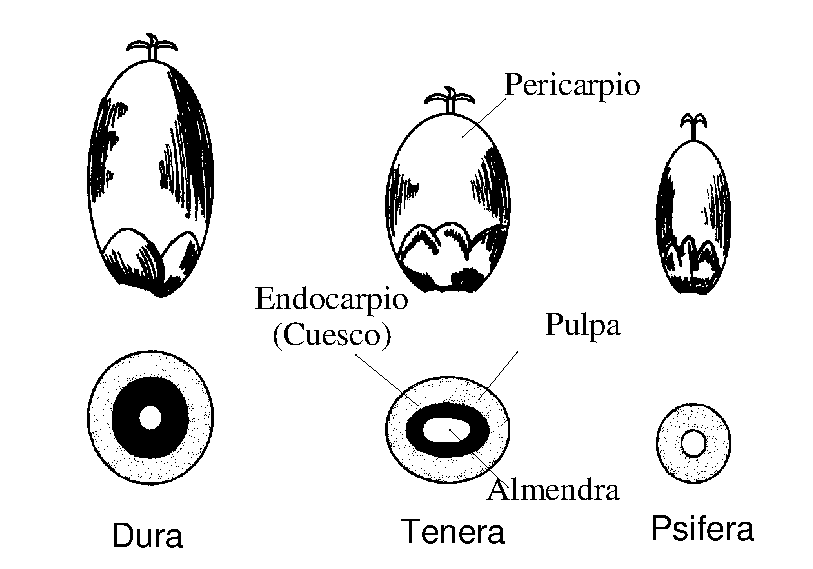
\includegraphics{Kap3/FrutoSp}%
\caption{Tipos y partes del fruto de palma de aceite \cite{AG03p,AG04p}.} \label{fig:Fruto}
\end{figure}

\section{Etapa 2}
Para la edici\'{o}n de tablas, cada columna debe llevar su t\'{\i}tulo; la primera palabra se debe escribir con may\'{u}scula inicial y preferiblemente sin abreviaturas. En las tablas y cuadros, los t\'{\i}tulos y datos se deben ubicar entre l\'{\i}neas horizontales y verticales cerradas (como se realiza en esta plantilla).\\

\subsection{Requerimientos}


\subsection{C\'alculos/dimensionamiento}

\subsection{Desarrollo }
La numeraci\'{o}n de las tablas se realiza de la misma manera que las figuras o ilustraciones, a lo largo de todo el texto. Deben llevar un t\'{\i}tulo breve, que concreta el contenido de la tabla; \'{e}ste se debe escribir en la parte superior de la misma. Para la presentaci\'{o}n de cuadros, se deben seguir las indicaciones dadas para las tablas.\\

Un ejemplo para la presentaci\'{o}n y citaci\'{o}n de tablas (citaci\'{o}n indirecta), se presenta a continuaci\'{o}n:\\

De esta participaci\'{o}n aproximadamente el 60 \% proviene de biomasa
(Tabla \ref{EMundo1}).
\begin{center}
\begin{threeparttable}
\centering%
\caption{Participaci\'{o}n de las energ\'{\i}as renovables en el suministro
total de energ\'{\i}a primaria \cite{AG02i}.}\label{EMundo1}
\begin{tabular}{|l|c|c|}\hline
&\multicolumn{2}{c|}{Participaci\'{o}n en el suministro de energ\'{\i}a primaria /\% (Mtoe)\;$\tnote{1}$}\\\cline{2-3}%
\arr{Region}&Energ\'{\i}as renovables &Participaci\'{o}n de la biomasa\\\hline%
Latinoam\'{e}rica&28,9 (140)&62,4 (87,4)\\\hline%
\:Colombia&27,7 (7,6)&54,4 (4,1)\\\hline%
Alemania&3,8 (13,2)&65,8 (8,7)\\\hline%
Mundial&13,1 (1404,0)&79,4 (1114,8)\\\hline
\end{tabular}
\begin{tablenotes}
\item[1] \footnotesize{1 kg oe=10000 kcal=41,868 MJ}
\end{tablenotes}
\end{threeparttable}
\end{center}

NOTA: en el caso en que el contenido de la tabla o cuadro sea muy extenso, se puede cambiar el tama\~{n}o de la letra, siempre y cuando \'{e}sta sea visible por el lector.\\

* Etapa 3
** Requerimientos
** Cálculos/dimensionamiento

** Desarrollo

** Herramientas

** Hardware
** Software

* Resultados y discusión




\chapter{Marco Conclusivo}
\section{Conclusiones}
Las conclusiones constituyen un cap\'{\i}tulo independiente y presentan, en forma l\'{o}gica, los resultados de la tesis  o trabajo de investigaci\'{o}n. Las conclusiones deben ser la respuesta a los objetivos o prop\'{o}sitos planteados. Se deben titular con la palabra conclusiones en el mismo formato de los t\'{\i}tulos de los cap\'{\i}tulos anteriores (T\'{\i}tulos primer nivel), precedida por el numeral correspondiente (seg\'{u}n la presente plantilla).\\

\section{Recomendaciones}
Se presentan como una serie de aspectos que se podr\'{\i}an realizar en un futuro para emprender investigaciones similares o fortalecer la investigaci\'{o}n realizada. Deben contemplar las perspectivas de la investigaci\'{o}n, las cuales son sugerencias, proyecciones o alternativas que se presentan para modificar, cambiar o incidir sobre una situaci\'{o}n espec\'{\i}fica o una problem\'{a}tica encontrada. Pueden presentarse como un texto con caracter\'{\i}sticas argumentativas, resultado de una reflexi\'{o}n acerca de la tesis o trabajo de investigaci\'{o}n.\\

\section{Trabajo Futuro}

\addcontentsline{toc}{chapter}{\numberline{}Bibliograf\'{\i}a}
\bibliographystyle{plaindin_esp}
\bibliography{BibliMSc}
\bibliography{mendeleybib}
\begin{appendix}
\chapter{Anexo: Nombrar el anexo A de acuerdo con su contenido}\label{AnexoA}
Los Anexos son documentos o elementos que complementan el cuerpo de la tesis o trabajo de investigaci\'{o}n y que se relacionan, directa o indirectamente, con la investigaci\'{o}n, tales como acetatos, cd, normas, etc.\\

\chapter{Anexo: Nombrar el anexo B de acuerdo con su contenido}
A final del documento es opcional incluir \'{\i}ndices o glosarios. \'{E}stos son listas detalladas y especializadas de los t\'{e}rminos, nombres, autores, temas, etc., que aparecen en el mismo. Sirven para facilitar su localizaci\'{o}n en el texto. Los \'{\i}ndices pueden ser alfab\'{e}ticos, cronol\'{o}gicos, num\'{e}ricos, anal\'{\i}ticos, entre otros. Luego de cada palabra, t\'{e}rmino, etc., se pone coma y el n\'{u}mero de la p\'{a}gina donde aparece esta informaci\'{o}n.\\

\chapter{Anexo: Nombrar el anexo C de acuerdo con su contenido}
MANEJO DE LA BIBLIOGRAF\'{I}A: la bibliograf\'{\i}a es la relaci\'{o}n de las fuentes documentales consultadas por el investigador para sustentar sus trabajos. Su inclusi\'{o}n es obligatoria en todo trabajo de investigaci\'{o}n. Cada referencia bibliogr\'{a}fica se inicia contra el margen izquierdo.\\

La NTC 5613 establece los requisitos para la presentaci\'{o}n de referencias bibliogr\'{a}ficas citas y notas de pie de p\'{a}gina. Sin embargo, se tiene la libertad de usar cualquier norma bibliogr\'{a}fica de acuerdo con lo acostumbrado por cada disciplina del conocimiento. En esta medida es necesario que la norma seleccionada se aplique con rigurosidad.\\

Es necesario tener en cuenta que la norma ISO 690:1987 (en Espa\~{n}a, UNE 50-104-94) es el marco internacional que da las pautas m\'{\i}nimas para las citas bibliogr\'{a}ficas de documentos impresos y publicados. A continuaci\'{o}n se lista algunas instituciones que brindan par\'{a}metros para el manejo de las referencias bibliogr\'{a}ficas:\\

\begin{center}
\centering%
\begin{tabular}{|p {7.5 cm}|p {7.5 cm}|}\hline
\arr{Instituci\'{o}n}&Disciplina de aplicaci\'{o}n\\\hline%
Modern Language Association (MLA)&Literatura, artes y humanidades\\\hline%
American Psychological Association (APA)&Ambito de la salud (psicolog\'{\i}a, medicina) y en general en todas las ciencias sociales\\\hline
Universidad de Chicago/Turabian &Periodismo, historia y humanidades.\\\hline
AMA (Asociaci\'{o}n M\'{e}dica de los Estados Unidos)&Ambito de la salud (psicolog\'{\i}a, medicina)\\\hline
Vancouver &Todas las disciplinas\\\hline
Council of Science Editors (CSE)&En la actualidad abarca diversas ciencias\\\hline
National Library of Medicine (NLM) (Biblioteca Nacional de Medicina)&En el \'{a}mbito m\'{e}dico y, por extensi\'{o}n, en ciencias.\\\hline
Harvard System of Referencing Guide &Todas las disciplinas\\\hline
JabRef y KBibTeX &Todas las disciplinas\\\hline
\end{tabular}
\end{center}

Para incluir las referencias dentro del texto y realizar lista de la bibliograf\'{\i}a en la respectiva secci\'{o}n, puede utilizar las herramientas que Latex suministra o, revisar el instructivo desarrollado por el Sistema de Bibliotecas de la Universidad Nacional de Colombia\footnote{Ver: www.sinab.unal.edu.co}, disponible en la secci\'{o}n "Servicios", opci\'{o}n "Tr\'{a}mites" y enlace "Entrega de tesis".

\end{appendix}

\end{document}
\end{document}